\documentclass[11pt,a4paper,oneside]{memoir}

\usepackage[utf8]{inputenc} 
\usepackage[T1]{fontenc}
\usepackage[french]{babel}
\usepackage{amsmath}
\usepackage{amsthm}
\usepackage{amssymb,amsthm,amsfonts}
\usepackage{url,color}
\usepackage{listings}
% -----------
% Pour la couleur dans les zones de code source (lstlisting)
% cf https://en.wikibooks.org/wiki/LaTeX/Source_Code_Listings
\usepackage{xcolor}
\lstdefinestyle{customc}{
  belowcaptionskip=1\baselineskip,
  breaklines=true,
  frame=L,
  xleftmargin=\parindent,
  language=C,
  showstringspaces=false,
  basicstyle=\footnotesize\ttfamily,
  keywordstyle=\bfseries\color{green!40!black},
  commentstyle=\itshape\color{purple!40!black},
  identifierstyle=\color{blue},
  stringstyle=\color{orange},
}
\lstset{escapechar=@,style=customc}
% ----------
\usepackage{graphicx}
\usepackage{geometry}
\usepackage{calc}
\usepackage{hyperref}

\geometry{hmargin=2cm,vmargin=2.5cm}

\setcounter{secnumdepth}{10}
\setcounter{tocdepth}{10}


%c'est pour avoir N, Z, Q, R, C
\newcommand{\R}{\mathbb{R}}	\newcommand{\Q}{\mathbb{Q}}	\newcommand{\C}{\mathbb{C}}
\newcommand{\N}{\mathbb{N}}	\newcommand{\Z}{\mathbb{Z}}


\theoremstyle{definition}
\newtheorem{definition}{Définition}

\theoremstyle{remark}
\newtheorem*{remarque*}{{Remarque}}

\theoremstyle{plain}
\newtheorem{proposition}{{Proposition}}
\newtheorem*{proposition*}{{Proposition}}
\newtheorem{theorem}{{Théorème}}



%\title{}
%\author{}
%\date{}


\begin{document}
%\maketitle


% ------------- Page de garde ------------------
\thispagestyle{empty}

\begin{minipage}{.47\textwidth}
\centering
\begin{flushleft}

\includegraphics[scale=0.25]{./Images-Rapport/logo_uvsq.jpeg}
\end{flushleft}
\end{minipage}
\begin{minipage}{.47\textwidth}
\centering
\begin{flushright}
\hspace*{1cm} 
\includegraphics[scale=0.9]{./Images-Rapport/logo_saclay.jpeg}
\end{flushright}
\end{minipage}


\begin{center}
\huge
\textbf{Master 1\\ Calcul Haute Performance et Simulation}
\end{center}


\begin{center}
  \vspace*{\stretch{3}}
  \hrule
  \hrule
  ~\\
  \begin{center}
    \huge
    \textbf{Rapport de stage}\\
    \bigskip
    \textbf{\'Evaluation de performances via des mini-applications}\\
  \end{center}
  ~\\
  \hrule
  \hrule
\end{center}

\vspace*{\stretch{2}}

\begin{center}
	\Large
	\textsc{\textbf{Stagiaire :}}\\
	\textsc{Robin CAZALBOU}\\
	~ \\
	\textsc{\textbf{Encadrant universitaire :}}\\
	\textsc{Pablo OLIVEIRA}\\
	~ \\
	\textsc{\textbf{Tuteur du Centre Borelli :}}\\
	\textsc{Fikri HAFID}\\
\end{center}

\begin{center}

\includegraphics[scale=0.22]{./Images-Rapport/logo_centre_borelli.png}
\end{center}

\vspace*{\stretch{5}}

\begin{center}
\textsc{\textbf{Année universitaire 2020-2021}}
\end{center}

% ----------------------------------------------





\newpage
\tableofcontents



\begin{vplace}[0.5]

\chapter*{Remerciements}
\addcontentsline{toc}{chapter}{Remerciements}

% texte à écrire ici
% fusionner remerciements et introduction




\chapter*{Introduction}
\addcontentsline{toc}{chapter}{Introduction}

% texte à écrire ici
Ce rapport tient compte des travaux que j'ai réalisé durant mon stage optionnel de fin de master 1 au centre Borelli de l'université Paris Saclay et de l'ENS Paris Saclay. Il fut réalisé sur la période du 17 mai au 28 août 2021, sous la tutelle de M. Fikri HAFID, chercheur au laboratoire du centre Borelli. \bigskip
~\bigskip

% travail en distanciel et en présentiel ?
% ressenti de ce que j'ai pu faire globalement pendant ce stage (premier résumé)

Le cœur de mon travail a consisté en l'étude des mini-applications d'une point de vue Calcul Haute Performance.

% ce que j'ai appris


\end{vplace}







\newpage


\chapter{\'Etat de l'art des mini-applications}

Dans un premier temps, faisons un premier tour d'horizon des mini-applications (que nous appellerons aussi miniapps).

\section{Qu'est ce qu'une miniapp ?}

Une mini-application est définie comme un code de calcul de petite taille (quelques milliers de lignes de code), compilé à partir d'un Makefile simple, cela dans le but de permettre une compréhension plus rapide de l'anatomie interne du code de la part des développeurs \cite{sandia2009}. Ces codes opensource ont pour objectif d'effectuer des simulations simples de problèmes physiques à partir de cœurs d'algorithme de calculs.

Ainsi, la plupart des mini-applications sont obtenues à partir de code de plus grande envergure (par exemple miniXyce, qui simule des circuits électriques, est issue du code Xyce qui comporte plus de 500.000 lignes de codes \cite{sandia2009}). Cependant, contrairement à leur homologue de grande taille, les miniapps n'ont pas pour objectif principal de simuler des problèmes physiques complexes ou inatteignable analytiquement. En effet, la validation des résultats se fait par l'intermédiaire de solutions calculées de façon exacte. L'intérêt sur le résultat à proprement parler est donc infime.

Par ailleurs, les données obtenues après l'exécution du code sont contenues dans des fichiers au format YAML \cite{yaml}, qui possède l'avantage d'être lisible par un humain tout en stockant les informations pour une possible base de données. Des librairies de conception de fichiers au format YAML sont disponibles pour de nombreux langages de programmation.\bigskip

Afin d'être utiles à plusieurs acteurs du monde de la simulation et du Calcul haute performance, ces miniapps se présentent sous la forme simplifiée d'un ou plusieurs \underline{cœurs de calcul numérique}, chacun centré sur une étape clé de l'algorithme global. Par exemple, dans le cas de la mini-application miniFE (pour "mini Finite Elements"), l'étude est centrée sur une méthode des éléments finis, et plus particulièrement sur l'application d'un algorithme de gradient conjugué, qui peut faire l'objet de nombreuses améliorations.

Ces miniapps ont ainsi plusieurs objectifs :
\begin{itemize}
\item permettre aux développeurs HPC et aux numériciens de proposer des méthodes innovantes de communications au sein de l'algorithme, en écartant toutes les données superflues et en permettant une large marge de manœuvre pour effectuer des modifications,
\item permettre d'évaluer les performances d'une architecture de cluster de calcul en considérant la miniapp comme un benchmark simplifié,
\item permettre d'effectuer les modifications du code en conséquences afin de faire concorder matériel et algorithme.
\end{itemize}\bigskip



\section{Présentation de quelques miniapps}

Du fait de la grande diversité des origines des problèmes physiques, ainsi que des approches numériques pour les résoudre, le champs des mini-applications est très vaste. Le Sandia National Laboratories fut un des initiateurs du concept de mini-application et au travers notamment du projet Mantevo \cite{mantevo-project}, de nombreuses miniapps furent conçues. Dans la suite Mantevo 3.0 \cite{heroux2015}, nous pouvons ainsi trouver, entres autres, :
\begin{itemize}
\item \textbf{miniFE} (ou parfois appelée \textbf{HPCCG}) : une mini-application axée sur la résolution d'un système d'équation non-linéaire par la méthode des éléments finis. Le solveur (ou cœur de calcul du code) utilise la méthode du gradient conjugué. Il est écrit en langage C++ et utilise la notion de classe template pour permettre notamment l'étude de l'influence de différents types du C++ permettant le stockage des valeurs (float, double, et leurs variants). Des implémentations hybride MPI+OpenMP, CUDA, OpenCL.
\item \textbf{miniAero} (ajouté à la version 3.0 seulement) : une miniapp de résolution d'équations de Navier-Stokes compressibles, en utilisant des volumes finis au travers d'une méthode de Runge-Kutta d'ordre 4 \cite{miniaero-code}. Le code est écrit en C++.
\item \textbf{TeaLeaf} : écrite en Fortran avec des implémentations OpenMP, MPI et OpenCL, cette miniapp résout l'équation linéaire de la chaleur sur une grille 2D, en utilisant un stencil à 5 points (c'est-à-dire pour lequel chaque cellule mémoire a besoin des données contenues dans les 4 cellules adjacentes). Une version TeaLeaf3D est en développement pour étendre la résolution du problème à un stencil à 7 points. \cite{tealeaf}
\item \textbf{miniGhost} : écrite elle aussi en Fortran et proposant un stencil 5 points, miniGhost étudie notamment plusieurs paradigmes de communications inter-processus en proposant des implémentations sur le modèle BSPMA (Bulk Synchronous Parallel with Message Aggregation), qui consiste à effectuer une phase lourde en communications pendant un intervalle de temps compact, puis à passer à une phase composée uniquement de calculs. D'autres implémentations (SVAF, SVCP) sont proposées et permettent une étude approfondie de ce modèles et de leurs concordances avec l'architecture cible du calculateur \cite{barrett2012}.
\item et bien d'autres (\textbf{miniMD}, \textbf{miniXyce}, \textbf{PathFinder}, \textbf{CoMD}, ...) \cite{heroux2015}
\end{itemize}\bigskip


Afin de pouvoir travailler plus précisément sur le code d'une miniapp en particulier, il m'a fallut faire un choix parmi toutes celles proposées. J'ai écarté celles écrites en Fortran, qui m'auraient demandé un effort supplémentaire dans leur lecture, étant plus familier avec le langage C/C++. Mon choix s'est d'abord penché vers miniAero, dont la segmentation du code permettait une lecture agréable et simplifiée. Cependant l'implémentation proposée par le projet Mantevo \cite{miniaero-code} s'appuyait fortement sur une bibliothèque externe nommée Kokkos, qui exploite un paradigme de programmation du C++ par l'abstraction et l'utilisation massive de templates. Bien que miniAero reste une miniapp du fait que les composantes de Kokkos soient compilées à l'intérieur d'elle, la compréhension de sa structure devenait lourde et aurait impacté les efforts fournis pour comprendre les résultats des mesures effectuées, mais aussi pour éventuellement fournir des améliorations ou modifications du code.\bigskip

J'ai finalement choisi de me concentrer sur la mini-application \textbf{miniXyce}. Cette dernière est un proxy de Xyce, un simulateur de circuit électrique, construit avec un design modulaire et flexible en C++ \cite{xyce}. MiniXyce résout les problèmes linéaires non-symétriques qui apparaissent dans des circuits composés de bobines, de résistances et de condensateurs grâce à une généralisation de la méthode de minimisation des résidus (ou GMRES) et une méthode d'Euler implicite pour l'intégration du temps \cite{minixyce-code}.

Par ailleurs, suite à la sortie de la version 1.0.0 de miniXyce, les développeurs signalent que sa conception a été axée sur la vérification que les résultats retournés étaient corrects, mais que des "analyses approfondies de Xyce ont montré des problèmes de performance sur trois phases de la simulation : le parsing, le chargement/l'évaluation du device, et la solution des équations linéaires" \cite{minixyce-code}.









\chapter{\'Etude comparative de Xyce et miniXyce}

MiniXyce étant issue de Xyce, une étude comparative des deux applications nous permettra d'évaluer les résultats prédits par chacun ainsi que les performances obtenues.

\section{Installation des applications}

Tout d'abord, pour installer et compiler miniXyce à partir des codes sources, les étapes ont été très simples : le dépôt Github \cite{minixyce-code} propose l'ensemble du code source, contenant un Makefile ainsi que les fonctions de calcul, sans appel à une bibliothèque externe (autre que la bibliothèque standard). Un README d'une petite centaine de lignes présente l'ensemble de la miniapp, de son installation et de son utilisation. Cela ne prend que quelques minutes.

\underline{\textbf{Remarque :}} la version disponible sur Github en "release" est la 1.0.0, qui est celle étudiée dans \cite{minixyce-validation}. Plusieurs améliorations de la part de Thornquist ont ensuite été proposées pour obtenir une version 1.1 a priori mieux distribuée selon MPI. De plus, une implémentation utilisant la bibliothèque Kokkos est proposée (en supposant que cette dernière est pré-installée) : nous ne l'étudierons pas car elle dénature le principe de la miniapp, qui est de rester dissociée d'une quelconque bibliothèque externe. Cependant, les quelques essais que j'ai effectué, ainsi que l'analyse du code source, m'ont montré que la version 1.1 ne retourne que les mesures de temps de l'application. Aucun résultat sur le circuit électrique n'est retourné. En l'état, nous continuerons donc notre analyse de miniXyce sur la \textbf{version 1.0.0} .\bigskip


Pour Xyce, les codes sont aussi disponibles sur Github ou sur le site du Sandia National Laboratory \cite{xyce} avec plusieurs notices de plusieurs centaines de pages chacune expliquant en détail la configuration, l'installation et l'utilisation. Du fait de l'ampleur d'un tel code (SLOC $\simeq$ 370 k), la compilation de Xyce seul prend plusieurs dizaines de minutes. Il est à noter aussi que Xyce exploite plusieurs bibliothèques externes, dont BLAS/LAPACK (les bibliothèques d'algèbre linéaire optimisées), FFT, la suite Sparse, ainsi que Trilinos, une bibliothèque conçue aussi par le Sandia Laboratory, et prenant elle aussi plusieurs dizaines de minutes à compiler (après des efforts de configuration).\bigskip

Dans le contexte HPC ou dans l'étude numérique seule, nous pouvons déjà observer que si miniXyce a bien été conçue pour refléter le cœur de calcul de Xyce, son utilisation à la place de Xyce sera nettement plus facilitée.


\section{Résultats obtenus par les applications}

D'après les travaux de Aadithya, Keiter et Thornquist \cite{minixyce-validation}, les résultats obtenus par miniXyce ont pu être validés sur plusieurs circuits différents.

Dans l'ensemble de test de miniXyce 1.0.0, nous pouvons ainsi trouver 5 circuits, ainsi que des scripts de génération d'échelles RC (c'est-à-dire plusieurs condensateurs en parallèles séparés par des résistances) de tailles arbitrairement grande.
Ces 5 circuits représentent des cas simples :
\begin{itemize}
\item circuit 1 : deux couples de résistances branchées en parallèle,
\item circuit 2 : une échelle RC à deux échelons,
\item circuit 3 : un circuit RLC en série,
\item circuit 4 : un circuit RLC simple en parallèle,
\item circuit 5 : un autre circuit RLC plus complexe en parallèle (2 résistances).
\end{itemize}
De plus, différents types de générateurs de courant ou de tension sont utilisés. MiniXyce est réduite aux seuls composants R, L, C, V et I (pour résistance, bobine, condensateur, générateur de tension et générateur de courant respectivement) : nous passons ainsi en revue tous ces éléments.\bigskip

MiniXyce et Xyce fonctionnent tous les deux en ligne de commande (une interface graphique est possible pour Xyce mais n'a pas d'intérêt dans notre étude et ne ferait que ralentir les temps d'exécution). De plus, ils ne nécessitent qu'un seul fichier en entrée, le reste des arguments constitue des options (sur les conditions initiales ou l'instant de début de simulation par exemple). Le fichier, nommé "netlist", contient toutes les informations sur les composants et l'architecture du circuit étudié. Le code source de miniXyce comporte de base les netlists de test issus des observations de \cite{minixyce-validation} et représentant les circuits 1 à 5 présentés précédemment.

Par ailleurs, il est à noter que Xyce et miniXyce proposent une implémentation séquentielle et une autre parallèle. Il sera d'un premier abord intéressant de comparer les performances du cas séquentiel avec l'utilisation de MPI pour un seul processus (et quantifier l'overhead de MPI dans son utilisation en séquentiel).\bigskip


\subsection{Lancement de Xyce}

Le fonctionnement des netlists de Xyce demande beaucoup d'effort à être appréhendé, surtout lorsque l'on n'est pas expert en composants électriques. Je me suis donc basé sur les netlists de test de miniXyce pour reconstruire les netlists des 5 circuits pour Xyce. Que ce soit en version séquentielle ou parallèle, Xyce ressort les mêmes résultats pour un même circuit (comparaison effectuée avec la commande bash "diff").

Précisons au passage que les fonctionnalités de Xyce permettent d'afficher un grand nombre de types de résultats, mais que nous gardons seulement la mesure de la tension aux niveau des nœuds du circuit.

Les résultats obtenus par Xyce et fournis par les concepteurs de miniXyce étant nommés "gold standards", nous avons pu obtenir exactement ces valeurs pour les circuits 1, 2 et 4. Le circuit 5 n'a pas ses gold standards de fournis, et quant au circuit 3, nous avons observé une différence : cela est dû au fait que Xyce choisit elle-même les pas de temps qu'elle va prendre tout au long de l'étude, et seul un pas maximal peut être fixé. Il a donc fallu ruser en imposant à Xyce une liste d'instants de calcul de la tension du circuit. Cependant les valeurs pour ces instants sont obtenus à partir d'une interpolation sur les valeurs calculées selon le choix de Xyce.

Deux questions se posent alors :
\begin{itemize}
\item quel impact cette interpolation a-t-elle sur les performances de Xyce ?

En effet, nous forçons des valeurs spécifiques à être obtenues, et faisons entrer en jeu l'interpolation qui n'est pas disponible sous miniXyce. L'intérêt de l'étude de ce circuit en tant que tel semble ainsi plus limitée.
\item l'écart entre les deux fichiers de valeurs est-il grand ?

\'Etant donné que nous ne savons pas comment le gold standard du circuit 3 a été obtenu, nous devrons nous contenter de valeurs approchées.
\end{itemize}


\`A l'aide d'un petit code que j'ai conçu, nous pouvons ainsi mesurer les écarts des valeurs entre les deux fichiers, ce qui nous donne trois séries de données $S_1$, $S_2$ et $S_3$ (pour les tensions mesurées $V_1$, $V_2$ et $V_3$ en trois nœuds du circuit). Les moyennes et écarts-types calculés sont les suivants :
\begin{center}
\begin{tabular}{|c|c|c|c|}
\hline
Série de données (écarts) & $S_1$ & $S_2$ & $S_3$\\ \hline
Moyenne & $0.000472208$ & $0.000547048$ & $0.000313002$ \\ \hline
\'Ecart-type & $0.000328526$ & $0.000371713$ & $0.000232592$ \\ \hline
\end{tabular}
\end{center}

Nous voyons ainsi que l'interpolation nous donne des résultats très similaires. Il serait intéressant de mesurer l'impact de ce calcul supplémentaire sur le temps d'exécution du code.




\subsection{Lancement de miniXyce}

Précisons qu'avec la version 1.1 de miniXyce, les netlists Xyce sont acceptés (les commandes d'analyses plus poussées sont simplement ignorées par la miniapp). Ce n'est pas le cas pour la version 1.0.0 pour laquelle, par exemple, les commentaires sont symbolisés par un "\%" (là où Xyce les symbolise avec une "*").

Pour vérifier les résultats proposés par miniXyce, nous utilisons les scripts de tests qui sont proposés : ces derniers se basent sur les gold standards (que nous avons vérifié). Un script Perl compare le fichier de sortie Xyce avec le fichier de sortie miniXyce : les 4 circuits passent le test haut-la-main, avec une erreur moyenne sur chaque voltage d'au plus $10^{-10}$.

Les résultats de miniXyce sont plus complets que ceux de Xyce, étant donné qu'ils donnent à la fois le voltage et l'intensité, mais aussi le nombre d'itérations de la méthode GMRES et le nombre de "restarts".





\section{Premiers profils de performance}

Les deux applications présentent de base dans leur code une mesure du temps d'exécution, que ce soit le temps total de la simulation ou bien certaines sous-parties du code qui sont sensées prendre plus de temps.


\subsection{miniXyce}

En analysant le code de miniXyce, nous pouvons remarquer que les mesures de temps forment globalement une partition assez claire du temps total, mise à part sur la boucle principale. Nous trouvons ainsi les mesures de temps suivantes :
\begin{itemize}
\item le parsing des paramètres (conditions initiales, intervalles de temps de la simulation, ...)
\item le parsing du netlist (et donc de la structure du circuit modélisé, des composants en jeu)
\item le calcul du DC Operating Point (ou point de fonctionnement)
\item la mise en place d'une matrice (matrix set up)
\item des I/O pour le résultat de l'application (la tension sur les composants du circuit dans nos exemples)
\item les itérations sur la période transitoire (transient calculation)
\item et enfin la simulation dans son ensemble.
\end{itemize}

Il faut ajouter à cela d'infimes manipulations et allocations de variables entre les mesures (qui, du fait de leur prise de temps très faibles, ne seront pas pertinentes et peuvent être négligées), mais aussi dans le cas de MPI d'un bloc de 6 appels à MPI\_Allreduce, plutôt gourmand en temps.

Enfin, le temps d'exécution de la boucle principale est celui de la période transitoire. Cependant, chaque itération est ponctuée d'une communication inter-processus et d'un I/O de la part du processus 0 : ce temps est compté dans la mesure I/O. Il faut aussi y ajouter une première étape d'I/O avant le début de la période transitoire.

\begin{figure}[!ht]
\begin{center}
\includegraphics[scale=0.55]{Images-Rapport/schéma_miniXyce_1.0.0.png}
\caption{Schéma des différentes sous-parties du code de miniXyce 1.0.0, à partir des mesures de temps qui en sont faites. La partie Allreduce et ajout d'informations au document YAML n'est pas mesurée par la miniapp.}
\label{schéma_miniXyce_1.0.0}
\end{center}
\end{figure}

La figure \ref{schéma_miniXyce_1.0.0} schématise les différentes sous-parties dont la mesure de temps est effectuée de base par le code de miniXyce 1.0.0 .\bigskip

\`A partir de ces mesures, et afin d'avoir des résultat les plus stables possibles, j'ai conçu des scripts et petits codes permettant d'automatiser le lancement de la miniapp 10.000 fois : les résultats des mesures de temps sont récupérés et traités (calcul de moyenne, d'écart-type pour les barres d'erreurs, ainsi que pourcentage du temps par rapport au temps total total de la simulation), puis utilisés pour construire un histogramme résumant ces données (un script Gnuplot permet aussi d'automatiser le processus).\bigskip

\begin{figure}
\begin{center}
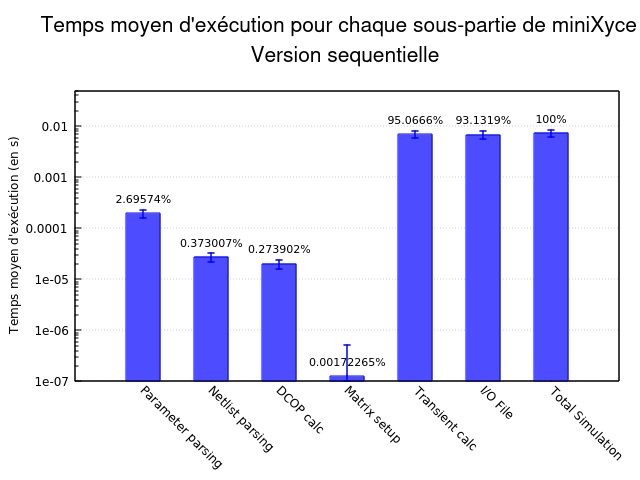
\includegraphics[scale=0.6]{Images-Rapport/Profil_miniXyce/Profil_miniXyce_sequentiel.png}
\caption{Profil simple de miniXyce, dans le cas séquentiel.}
\label{Profil_miniXyce_sequentiel}
\end{center}
\end{figure}

\begin{figure}
\begin{center}
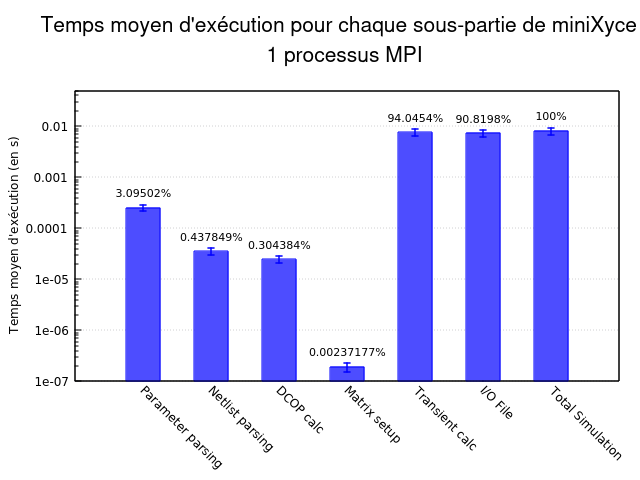
\includegraphics[scale=0.45]{Images-Rapport/Profil_miniXyce/Profil_miniXyce_parallele1.png}
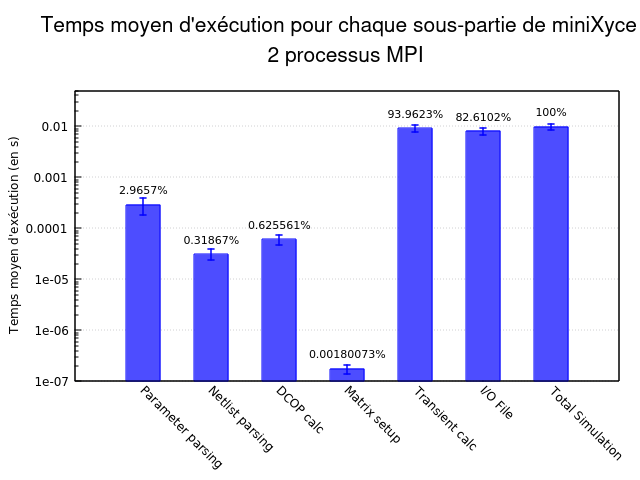
\includegraphics[scale=0.45]{Images-Rapport/Profil_miniXyce/Profil_miniXyce_parallele2.png}
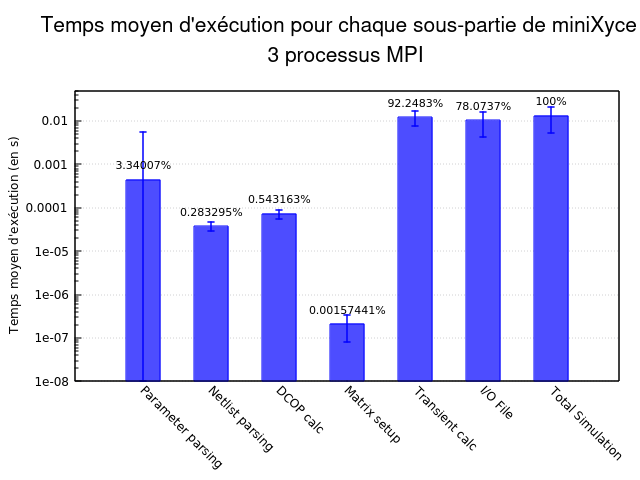
\includegraphics[scale=0.45]{Images-Rapport/Profil_miniXyce/Profil_miniXyce_parallele3.png}
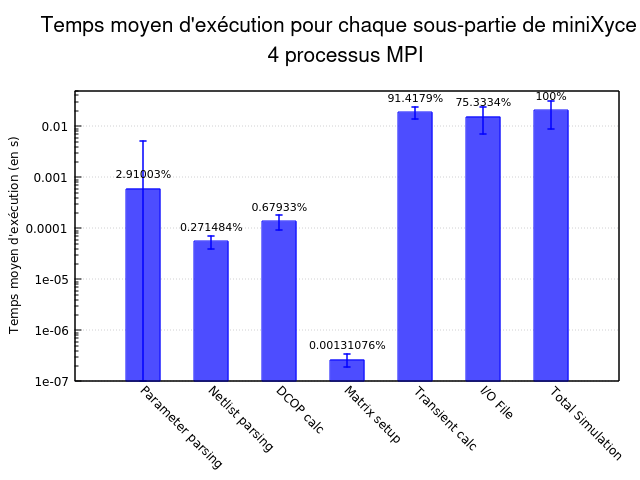
\includegraphics[scale=0.45]{Images-Rapport/Profil_miniXyce/Profil_miniXyce_parallele4.png}
\caption{Profils simples de miniXyce dans le cas parallèle, pour 1 à 4 processus MPI.}
\label{Profil_miniXyce_parallele}
\end{center}
\end{figure}

Nous retrouvons ainsi dans la figure \ref{Profil_miniXyce_sequentiel} les 7 mesures de temps présentées dans le schéma \ref{schéma_miniXyce_1.0.0}, en échelle logarithmique, et dans le cas séquentiel. Les pourcentages indiquent quelle proportion du temps total est prise par chaque sous-partie de miniXyce. Dans la figure \ref{Profil_miniXyce_parallele}, nous présentons les mêmes mesures dans le cas parallèle, et cela pour des tailles de communicateurs MPI allant de 1 à 4.

Précisons que toutes les mesures ont été faites en simulant les calculs sur le premier circuit présentés plus tôt dans ce chapitre. Ce circuit est très petit (seulement 4 résistances et une source de tension) et comporte peu d'intérêt physique. Cependant, il nous est très utile afin de tester les scripts proposés pour automatiser les mesures de temps et la conception d'un histogramme. Par ailleurs, nous nous proposons pour l'instant de fournir un premier profil du code, qui nous permettra de comprendre dans les grandes lignes les points chauds de miniXyce ainsi que ses faiblesses.

D'autre part, les mesures en multi-processus sont celles rapportées uniquement par le processus 0 : beaucoup de synchronisations sont encore présentes dans le code et les mesures se rapprochent de celles des autres processus. Ce n'est pas optimal pour notre étude, mais comme nous l'avons dit, nous présentons pour l'instant un premier profil simple.

Les mesures ont été réalisées sur ordinateur personnel (à mémoire partagée) à 4 cœurs hyperthreadés Intel i7-4700MQ (Haswell), et avec l'implémentation MPICH 3.4.1 pour MPI. Dans le cas parallèle, l'appel à MPI\_Wtime est utilisé pour les mesures de temps, alors que pour le cas séquentiel, c'est l'appel à gettimeofday qui est réalisé (sachant que sa précision est à la $\mu s$ près). Pour que gettimeofday soit utilisé, il a fallu faire une toute petite modification dans le code d'origine en ajoutant un flag de compilation (mais l'ensemble du code prenant déjà en charge gettimeofday, rien d'autre n'a été changé).\bigskip

La première chose à relever sur le profil de miniXyce est le fait que la somme des temps ne rejoint pas le temps de simulation total : cela s'explique par certains points du code non évalués, ainsi que par l'inclusion du temps d'I/O dans celui de la période de calcul transitoire.

Nous remarquons néanmoins que la proportion du temps des I/O diminue lorsque le nombre de processus augmente : étant donné que seul le processus 0 s'occupe des I/O, cette baisse est due au fait que le temps global augmente alors que les I/O restent constants. Les appels à MPI\_Allreduce doivent avoir un fort effet sur le temps d'exécution et montrent déjà une mauvaise scalabilité du code.

D'une manière générale, l'optimisation des I/O, la période transitoire et le parsing des paramètres semblent les plus chronophages et méritent le plus d'attention. Une remarque tout de même : notre circuit électrique étant pour l'instant très petit, il ne faut pas négliger la possibilité que la taille de la matrice explose avec le nombre de composants et que sa mise en place deviennent plus conséquente en temps : ce temps est donc à surveiller.




\subsection{Xyce}

Xyce propose de son côté des mesures plus détaillées et un rapport assez complet à la fin de l'exécution. Ne pouvant relire et comprendre tout le code de Xyce, je me suis contenté de récupérer les informations les plus globales afin de pouvoir comparer avec miniXyce, sans rentrer dans les détails complexes de mise en place des solveurs.

\begin{figure}
\begin{center}
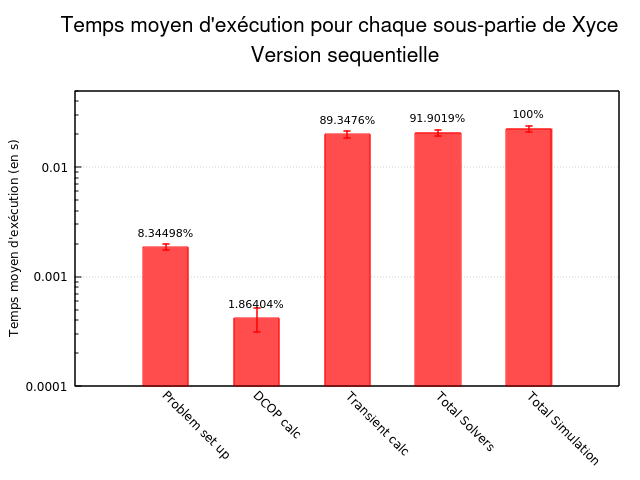
\includegraphics[scale=0.6]{Images-Rapport/Profil_Xyce/Profil_Xyce_sequentiel.png}
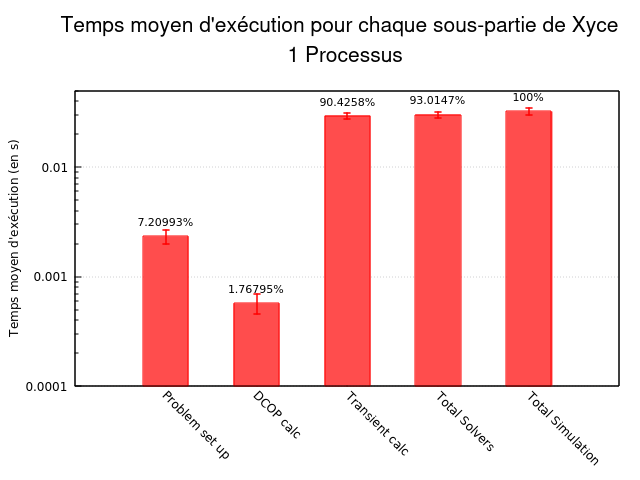
\includegraphics[scale=0.45]{Images-Rapport/Profil_Xyce/Profil_Xyce_parallele1.png}
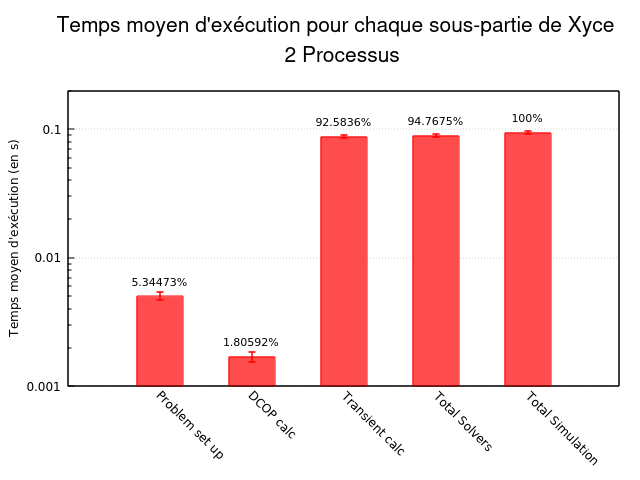
\includegraphics[scale=0.45]{Images-Rapport/Profil_Xyce/Profil_Xyce_parallele2.png}
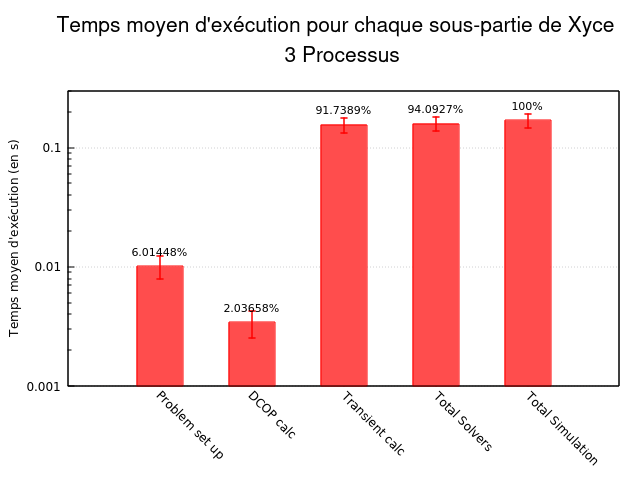
\includegraphics[scale=0.45]{Images-Rapport/Profil_Xyce/Profil_Xyce_parallele3.png}
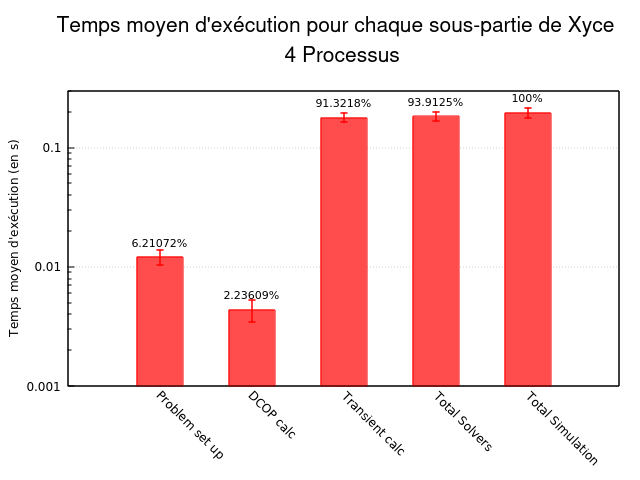
\includegraphics[scale=0.45]{Images-Rapport/Profil_Xyce/Profil_Xyce_parallele4.png}
\caption{Profil simple de Xyce, dans le cas séquentiel et dans le cas parallèle, pour 1 à 4 processus MPI.}
\label{Profil_Xyce}
\end{center}
\end{figure}


Nous présentons en figure \ref{Profil_Xyce} les profils obtenus avec Xyce, dans les mêmes circonstances que ceux obtenus avec la miniapp. Cinq mesures sont effectuées, dans lesquelles nous retrouvons le calcul DCOP, la période transitoire et le temps total de la simulation.

Les temps d'exécution globaux sont presque multipliés par 4, mais la période transitoire prend toujours dans les 90\% du temps, alors que le calcul DCOP reste dans les alentours de 1\%. Nous pouvons ainsi dire que les profils de performance des deux applications sont, a priori sur un circuit très simple, globalement similaire. MiniXyce présente ainsi l'intérêt d'approcher Xyce en se souciant de l'aspect performance. 









\chapter{Analyse approfondie de la miniapp}

Dans le précédent chapitre, nous avons donné un premier profil de miniXyce sur un circuit très petit à 4 résistances. Nous avons supposé que la scalabilité risquait d'être mauvaise, du fait d'I/O répétés mais aussi d'un partage de travail a priori déséquilibré.

Pour vérifier ou rejeter les hypothèses faites, il va nous falloir réaliser une étude plus approfondie se basant sur les points suivants :
\begin{itemize}
\item travailler sur un circuit de plus grande envergure, de sorte à ce que l'on puisse s'approcher d'un code de simulation plus réaliste et donc plus long en exécution. Nous pourrons refaire le profilage précédent et étudier les modifications.
\item travailler avec des outils de profiling plus fins comme Gprof ou Maqao
\item enfin, évaluer la scalabilité à proprement parlée (en se basant sur le temps total)
\end{itemize}



\section{Premières mesures et problématique du choix de version}

\`A partir des scripts Perl proposés dans le code source de miniXyce, j'ai décidé de générer des circuits plus gros sous la forme d'une échelle RLC à 100 échelons.

Ce choix est justifié par le fait que les premières expérimentations sur MAQAO ont nécessité un problème prenant au moins une seconde pour être résolu, afin que les mesures soient plus précises.

Les circuits peuvent être groupés selon les composants ou bien selon les échelons : en d'autres termes, il est possible de générer toute la liste des résistances, puis des condensateurs et enfin des bobines, ou bien créer une suite de R-C-L.\bigskip

Des mesures ont été refaites sur le profilage simple (cf figure \ref{profil_minixyce_v2}) ainsi qu'avec l'aide du module Oneview de MAQAO, qui offre une étude plus détaillée.

\begin{figure}
\begin{center}
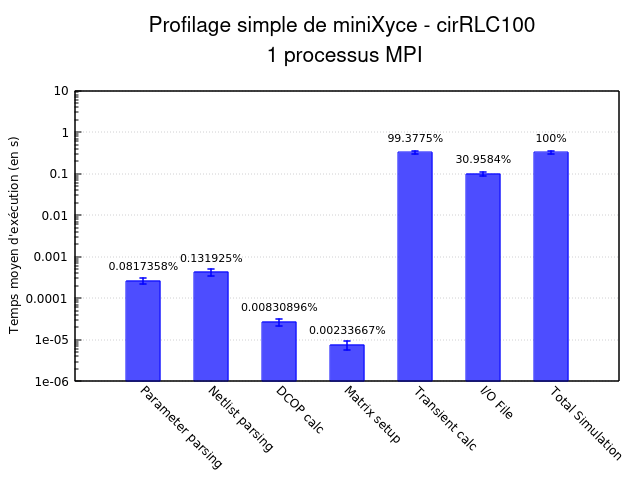
\includegraphics[scale=0.45]{Images-Rapport/Profil_miniXyce_v2/Profil_miniXyce_v2_1proc.png}
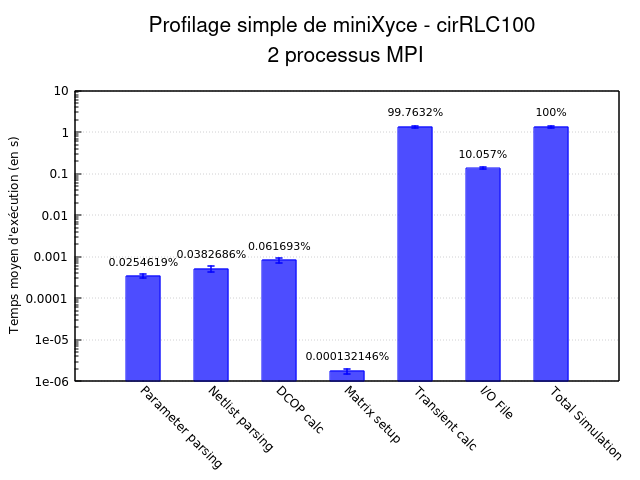
\includegraphics[scale=0.45]{Images-Rapport/Profil_miniXyce_v2/Profil_miniXyce_v2_2proc.png}
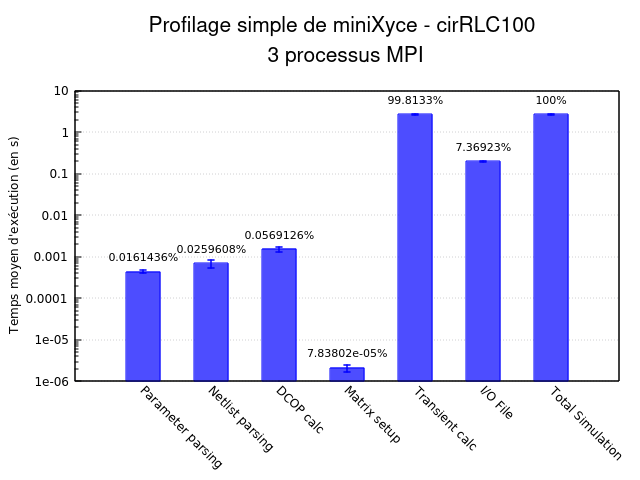
\includegraphics[scale=0.45]{Images-Rapport/Profil_miniXyce_v2/Profil_miniXyce_v2_3proc.png}
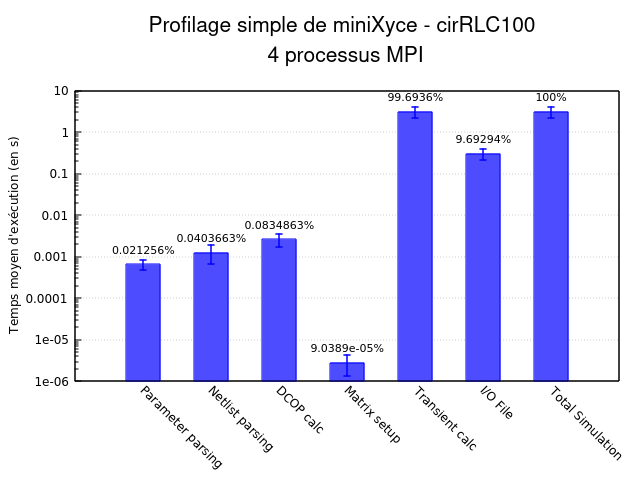
\includegraphics[scale=0.45]{Images-Rapport/Profil_miniXyce_v2/Profil_miniXyce_v2_4proc.png}
\caption{Deuxième profil simple de miniXyce pour plusieurs tailles de communicateur, sur le circuit RLC100.}
\label{profil_minixyce_v2}
\end{center}
\end{figure}

Pour le profil simple, nous pouvons observer d'une part que le temps de calcul DCOP prend petit à petit de l'importance, alors que le temps d'I/O réduit nettement, passant de 30\% à 9\%. Les autres quantités bougent peu.

Ce que ces échelles logarithmiques ne montrent pas, c'est que ces évolutions sont surtout marquées par le fait que le temps total a nettement augmenté. La figure \ref{profil_minixyce_v2_comparaison} compare ainsi les temps totaux : entre 1 et 4 processus, le temps d'exécution est presque multiplié par 10 !

\begin{figure}
\begin{center}
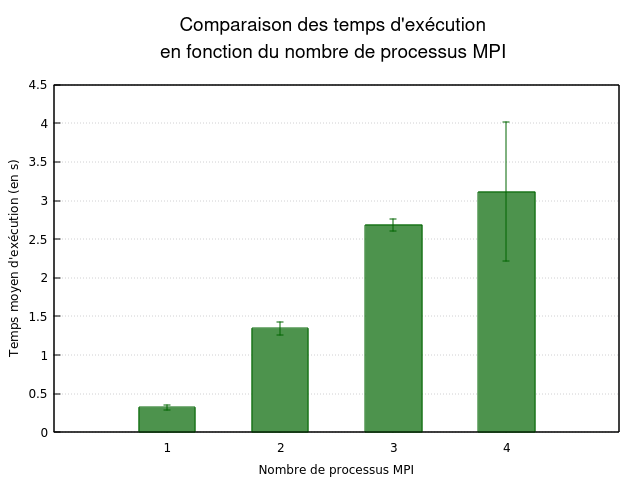
\includegraphics[scale=0.6]{Images-Rapport/Profil_miniXyce_v2/Comparaison_profil_v2.png}
\caption{Comparaison des temps totaux de 1 à 4 processus (sans échelle logarithmique)}
\label{profil_minixyce_v2_comparaison}
\end{center}
\end{figure}


En poursuivant les analyses avec MAQAO, toujours sur les 4 tailles de communicateur, nous obtenons les répartitions du temps total d'exécution selon le type d'appel de fonctions (cf figure \ref{maqao_minixyce_v1}). MAQAO retourne un rapport plus détaillé, mais au vu des résultats obtenus, nous n'en aurons pas besoin. En effet, les résultats sont très explicites et montrent que beaucoup de temps est perdu dans des appels MPI (jusqu'à 82\% à 3 et 4 processus).

\begin{figure}
\begin{center}
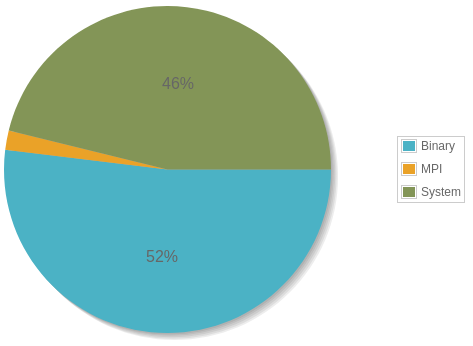
\includegraphics[scale=0.45]{Images-Rapport/MAQAO_V1/miniXyce_RLC100_1proc.png}
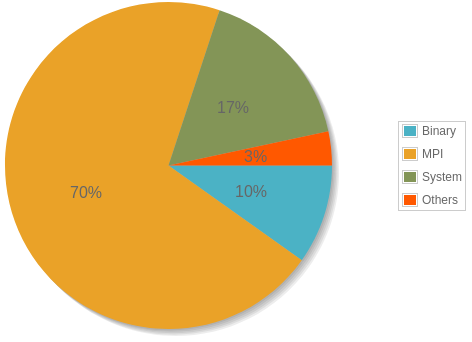
\includegraphics[scale=0.45]{Images-Rapport/MAQAO_V1/miniXyce_RLC100_2proc.png}
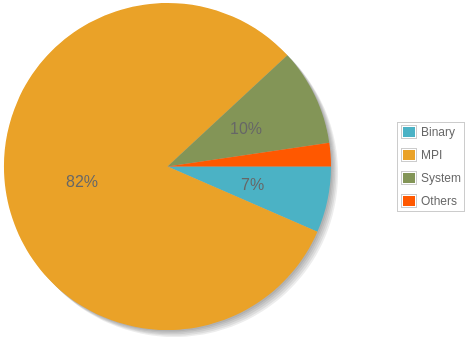
\includegraphics[scale=0.45]{Images-Rapport/MAQAO_V1/miniXyce_RLC100_3proc.png}
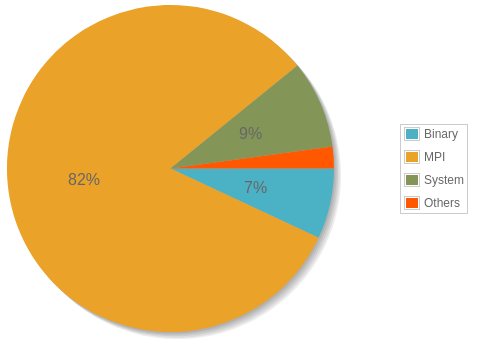
\includegraphics[scale=0.45]{Images-Rapport/MAQAO_V1/miniXyce_RLC100_4proc.png}
\caption{Répartitions du temps d'exécution suivant les types de fonctions, d'après MAQAO Oneview (haut gauche : 1 processus, haut droite : 2 processus, bas gauche : 3 processus, bas droite : 4 processus).}
\label{maqao_minixyce_v1}
\end{center}
\end{figure}


L'origine de ce pourcentage aussi élevé est assez incertaine. Nous constatons qu'il n'y a pas une concordance parfaite avec le profil simple que nous avons fait sans MAQAO : les I/O ne représentent plus une partie aussi importante (MAQAO ne les présente même pas, serait-ce dû à une mauvaise utilisation de l'outil ?).

Même si 6 appels successifs à Allreduce sont fait dans le code, ils ne représenteraient au maximum que 0.5\%. L'hypothèse que nous pouvons avancer est la suivante :
\begin{itemize}
\item la période transitoire est celle qui prend le plus de temps car elle appelle des fonctions de calculs coûteuses
\item elle doit aussi être mal organisée au niveau des communications MPI, ce qui expliquerait le taux relevé par MAQAO.
\end{itemize}\bigskip

% à ce stade, j'ai pensé à changer de version, mais...
\`A ce stade de mon étude, j'ai pensé à changer de version pour la 1.1 développée par Thornquist \cite{minixyce-code} à titre de comparaison. Et en effet, les résultats ont été bien plus satisfaisants pour la répartition, avec un taux des appels MPI à seulement 10\% pour 3 processus (cf figure \ref{maqao_minixyce_1.1}).

\begin{figure}
\begin{center}
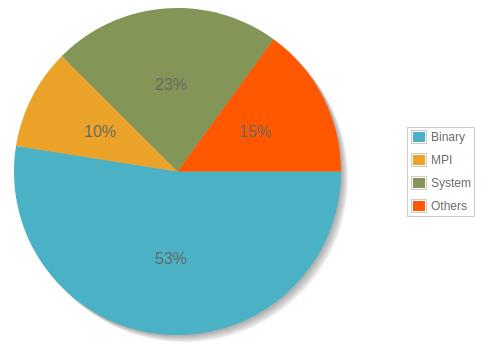
\includegraphics[scale=0.5]{Images-Rapport/maqao_minixyce_1.1_3proc.png}
\caption{Rapport MAQAO Oneview pour la version 1.1 de miniXyce, avec 3 processus.}
\label{maqao_minixyce_1.1}
\end{center}
\end{figure}

Rappelons que nous avions écarté la version 1.1 pour plusieurs raisons :
\begin{itemize}
\item tout d'abord, le release de la version 1.1 n'a pas été fait, mais seulement commité sur Github parmi d'autres améliorations proposées par Thornquist, ce qui laissait insinuer que la version 1.1 n'était qu'une ébauche (potentiellement non valide),
\item l'application ne retournait pas de résultats sur la tension dans le circuit,
\item son rapport YAML (profil des temps) comporte de nouvelles entrées (residual load time, jacobian load time, jacobian assembly time) mais ne précise plus le temps total.
\end{itemize}

J'ai donc analysé en détails le code source afin de voir s'il était possible de rajouter les résultats et la mesure du temps total. Cependant, après examen des commits, j'ai laissé cette idée de côté car de nombreuses modifications sur les méthodes de distribution des vecteurs parmi les processus ont été mises en place, et le solveur même ne semblait plus être le cœur de l'étude (le parsing et la généricité des classes modélisant les appareils électroniques ont primé).

Nous poursuivrons notre analyse en essayant de corriger la version 1.0, plutôt qu'en "annulant" des ajouts de la 1.1 .






\section{Un peu de génie logiciel}

La version de miniXyce 1.0.0 possède le désavantage d'avoir un Makefile supprimant les versions antérieures de l'exécutable, même si celui-ci est en séquentiel alors que l'on cherche à compiler en parallèle (et inversement). J'ai commencé par le modifier afin d'avoir deux versions qui puissent coexister, et que des dossiers soient générés pour séparer fichiers objets et exécutables. Il est ainsi possible de compiler successivement avec "\textbf{make}", puis avec "\textbf{make -f Makefile.gnu.serial -B}" pour obtenir les deux versions (l'option -B force la recompilation des fichiers objets qui seraient prévus pour une version parallèle).

Par ailleurs, le script de lancement des mesures du profil simple a été étoffé de sorte à effectuer aussi le traitement en automatique, et à être plus générique, sans avoir à modifier le code source selon les choix de mesures (tailles de communicateurs MPI étudiées, nombre de répétitions).

Enfin, deux warnings, hérités du code d'origine (et ayant subsistés à chaque commit du dépôt officiel...) ont été corrigés : 
\begin{itemize}
\item le premier indiquait que le code de retour d'un appel système de création de dossier n'était pas pris en compte. Il a suffit d'ajouter une condition \textit{if} et un message d'erreur pour le régler.
\item le deuxième était plus fin et précisait qu'un buffer d'écriture était potentiellement trop petit pour contenir tous les caractères imposés. En comptant le nombre théorique minimum d'octets nécessaires, j'ai pu régler ce deuxième warning en agrandissant le buffer.
\end{itemize}


\section{Recherche des fonctions chronophages}

\'Etant donné que plus de 99\% du temps d'exécution est pris par la période transitoire, mais que seulement 10\% (à partir de 2 processus) est pris par les I/O, la perte de temps due aux appels MPI se situe dans une zone précise de la fonction \textit{main} : nous l'appellerons "zone critique MPI" :

\begin{lstlisting}
trans_steps++;

std::vector<double> b = evaluate_b(t,dae);

std::vector<double> RHS;
sparse_matrix_vector_product(B,x,RHS);

for (int i = 0; i < num_my_rows; i++)
{
	RHS[i] /= t_step;
	RHS[i] += b[i];
}

gmres(A,RHS,x,tol,res,k,x,iters,restarts);

total_gmres_iters += iters;
total_gmres_res += res;
\end{lstlisting}

Ce code étant situé dans une boucle \textit{while}, il est répété autant de fois qu'il y a de pas de temps choisis pour la simulation.

Dans cette zone critique, une boucle effectue seulement des opérations arithmétiques simples sur un vecteur, et trois fonctions sont appelées :
\begin{itemize}
\item \textbf{\textit{evaluate\_b}} : cette fonction, définie dans mX\_linear\_DAE.cpp, ne fait que des accès et modifications sur un vecteur, sans appels MPI,
\item \textbf{\textit{sparse\_matrix\_vector\_product}} : définie dans mX\_sparse\_matrix.cpp, elle consiste simplement à calculer le produit matrice-vecteur $A\times x$, dans le cas où $x$ est distribué entre les processus, et $A$ est creuse, linéarisée sous forme de liste chaînée et distribuée elle aussi entre les processus (par blocs de lignes). Elle effectue de nombreux envois/réceptions avec MPI\_Send/MPI\_Recv,
\item \textbf{\textit{gmres}} : définie aussi dans mX\_sparse\_matrix.cpp, elle résout un système linéaire par la méthode itérative GMRES. Elle fait elle-même appel à \textit{sparse\_matrix\_vector\_product} à 3 reprises, dont 2 à l'intérieur de boucle \textit{while}, ainsi qu'à MPI\_Allreduce. Elle appelle aussi la fonction \textbf{\textit{norm}} qui calcule une norme sur un vecteur distribué entre processus (notamment grâce à un MPI\_Allreduce).
\end{itemize}

Au vu de cette analyse, les trois fonctions \textbf{\textit{sparse\_matrix\_vector\_product}}, \textbf{\textit{gmres}} et \textbf{\textit{norm}} sont susceptibles de causer des ralentissements dans les communications et synchronisations inter-processus.\bigskip

Pour mesurer cela un peu plus finement, j'ai conçu de petites coroutines qui ont pour seul objectif de stocker dans une variable "static" le temps cumulé passé dans chacune des fonctions. Combiné avec le timer utilisé dans le code, nous pouvons ainsi obtenir le pourcentage du temps total d'exécution passé dans chacune des trois fonctions (et cela pour chaque processus).

Ce que l'on observe alors, c'est que pour un seul processus MPI, le temps d'I/O est de l'ordre de 45\% du temps total, et celui de \textit{gmres} est aux alentours de 54\% (dont 17\% passé dans la multiplication matrice-vecteur).

En passant à 4 processus, le temps d'exécution est déjà multiplié par 25 (passant de 3.1 à 78 s !) et la part d'I/O passe en dessous des 3\% pour le processus 0. Certains processus passent alors presque 99\% du temps dans la multiplication matrice-vecteur appelée par \textit{gmres}. Une disparité très forte apparaît alors sur les mesures, ce qui nous amène à la conclusion que les processus passent le plus clair de leur temps à attendre un autre processus pour une synchronisation.


% Il faudra ensuite faire un traitement (en modifiant le code que j'avais écris) + faire un graphique comparatif + analyser et dire sur quelle fonction il faudra qu'on fasse des efforts



\section{Première optimisation efficace}

Détaillons la façon dont \textit{sparse\_matrix\_vector\_product} est implémentée. Tout d'abord, elle se base sur une structure de matrice creuse distribuée entre processus :
\begin{itemize}
\item chaque processus possède un certain nombre de lignes de la matrice,
\item chaque ligne est caractérisée par un pointeur vers le premier "bloc valeur" de la ligne. Ces "blocs valeurs" (appelés \textit{distributed\_sparse\_matrix\_entry}) stockent l'indice de la colonne ainsi que la valeur de la matrice contenue sur cette ligne et cette colonne. Chaque "bloc valeur" contient aussi un pointeur vers le bloc suivant de la ligne, ce qui constitue une liste chaînée,
\item chaque processus connaît ainsi son indice de début et de fin des lignes qui lui sont attribuées. La distribution de la matrice est donc réalisée, et pour modéliser une matrice creuse, nous gagnons en efficacité de stockage.
\end{itemize}

Cependant, tout au long de l'application, une opération matricielle intervient : la multiplication matrice-vecteur. Or, avec le découpage proposé, chaque processus ne connaît du vecteur qu'une sous-partie associée aux lignes qui lui ont été attribuées. Des communications sur les autres valeurs du vecteur sont alors nécessaires. Prenons l'exemple suivant (fictif) de calcul du produit $Ax$ :

\[
A =
\begin{pmatrix}
0 & -1 & 0 & -2\\
0 & 3 & 0 & 0\\
0 & 0 & 1 & 0\\
6 & 0 & 0 & 3\\
\end{pmatrix} \quad \text{et} \quad
x = 
\begin{pmatrix}
1\\
2\\
3\\
4
\end{pmatrix}
\]

La distribution entre processus est telle que P0 possède les deux premières lignes et P1 les deux suivantes. Lorsque P0 voudra calculer la première coordonnée de $Ax$, il devrait calculer : $(-1) * 2 + (-2) * 4$. Mais P0 ne connaît pas la valeur $4$ car elle ne fait pas partie des deux premières lignes : un envoi de cette valeur de la part de P1 est nécessaire pour pouvoir ensuite faire le calcul. Il en est de même avec la valeur 1 à envoyer à P1, lorsqu'il voudra calculer la dernière composante de $Ax$ ($6*1+3*4$, la valeur 1 n'étant pas dans les lignes de $x$ qu'il possède).

Ainsi, avec ce stockage, il faut effectuer $n(n-1)$ échanges de messages dans le pire cas (chaque processus devant envoyer un message à tous les autres), soit une complexité en messages en $O(n^2)$ avec $n \in \N^*$ la taille de la matrice.\bigskip

Pour que chaque processus sache à qui il doit envoyer telle ou telle valeur, une autre structure contenant toutes ces informations est conservée et construite en même temps que la matrice. Ainsi, lors de la multiplication matrice-vecteur, dès qu'un processus ne possède pas la valeur dont il a besoin, il se met en position de réception de message et stockera la valeur temporairement pour toute la durée de la multiplication matrice-vecteur.\bigskip

\textbf{\underline{Problématique soulevée :}} avec ce schéma de communications, le code d'origine proposait un envoi de message \textbf{par valeur}. Ainsi, le nombre d'échanges pouvait être multiplié par un facteur compris entre 2 et $\frac{(N-1)n}{N}$ (selon la répartition des valeurs non nulles sur les lignes), ce qui donnait de l'ordre de $O(n^3)$ échanges de messages.

Précisons par ailleurs que les envois sont faits massivement dès le début de l'appel de la fonction, ce qui fait que tout processus attendant un message finira tôt ou tard par avoir ce qu'il attend.\bigskip

\textbf{\underline{Solution proposée :}} pour réduire les envois, lors de la phase de conception des messages, nous remplissons par processus un "buffer" contenant toutes les valeurs attendues. Un processus s'étant aperçu qu'il lui manquait une valeur devrait alors sonder (avec MPI\_Probe) pour déterminer si un message est en attente pour lui. Lorsque c'est le cas, il récupère la taille du message et, grâce à un "buffer" temporaire de réception, il stocke toutes ces valeurs dont il aura forcément besoin à un moment dans une \textit{std::map} (dictionnaire clé-valeur avec la clé étant l'indice de la composante du vecteur $x$). Ne sachant pas à l'avance quel processus doit lui envoyer la valeur attendue actuellement, une boucle \textit{while} effectue la vérification : si la valeur n'est pas encore dans la map, c'est que l'on a reçu d'un autre processus. Qu'à cela ne tienne, il aurait fallut récupérer cette valeur de toute façon. Lorsque la bonne valeur est enfin récupérée, le calcul se poursuit.

Nous pouvons alors observer, pour le circuit cirRLC1000 notamment, que le temps d'exécution à 4 processus redescend en dessous des 5 secondes. Ce temps reste plus long que celui en séquentiel, mais cela constitue tout de même une accélération d'un facteur 15 par rapport aux 78 secondes avant modification.

\textit{\underline{Remarque :}} un inter-blocage est envisageable avec cette amélioration lorsque la taille du système devient importante. En effet, les envois bufferisés deviendront des envois synchrones, et comme les réceptions ne se font qu'après tout les envois réalisés, le programme va bloquer. Une idée serait de grouper les réceptions en décidant par exemple que tous les processus de rang pair fassent leur réception d'abord. Cependant, comme chaque processus n'a connaissance de la valeur qu'il lui manque que lorsque qu'il fait des calculs, cette méthode casserait complètement le parallélisme.

Il faudrait alors modifier la structure de la matrice de sorte à ce que chaque processus sache à l'avance à qui il doit envoyer une valeur, mais aussi de qui (et donc combien) il doit en recevoir. Dans ce cas, le stockage de la matrice devient plus conséquent, mais le gain en temps devrait contre-balancer cette perte. Il faudrait dans ce cas utiliser des communications non-bloquantes pour couvrir au maximum les échanges par du calcul.\bigskip

\textbf{\underline{Direction à suivre :}} pour que notre programme passe encore mieux à l'échelle, il va être nécessaire de réduire encore plus les phases de synchronisations :
\begin{itemize}
\item Dans \textbf{gmres}, qui reste le cœur du solveur, beaucoup de communications avec l'ensemble des processus sont réalisées, qu'il faudra essayer d'\textbf{agencer différemment},
\item La remarque précédente peut aussi être prise en compte afin de voir si le coût de la multiplication matrice-vecteur peut encore être diminué,
\item Enfin, les I/O, bien que moins consistants dans le temps de certains processus, prennent tout de même toujours 30\% du temps du processus 0 (qui est le seul à faire les I/O). Nous pouvons ainsi penser que le temps d'attente des autres processus est accentué du fait de ce partage non équitable du travail : il faudrait alors paralléliser les I/O.
\end{itemize}




\chapter{Deuxième optimisation MPI et utilisation de Scalasca}

Dans le chapitre précédent, nous avons vu qu'une utilisation réduite des appels MPI avait permis de réduire drastiquement le temps d'exécution du programme pour un nombre de processus MPI supérieur ou égal à 2. Cependant, le temps restait toujours plus long que celui en séquentiel, ce qui indiquait que les communications restaient trop lourdes par rapport au temps gagné sur les calculs.

Nous avons aussi vu qu'un possible blocage pouvait apparaître si les tailles de buffer d'envoi devenaient trop grosses. La solution relevée était de changer l'ordre envoi/réception selon le rang du processus : au vu de la complexité possible de la matrice, cette solution ne serait pas bénéfique car trop de processus attendraient que d'autres aient terminé leurs envois.

Il reste ainsi une possibilité non exploitée : celle des communications non-bloquantes de type MPI\_Isend ou MPI\_Irecv. Leur utilisation va cependant nécessiter de nombreuses modifications dans les structures de données ainsi que dans l'écriture des algorithmes.


\section{Nouvelle écriture de la fonction du produit matrice-vecteur}

La nouvelle écriture de la fonction \textit{sparse\_matrix\_vector\_product} que je propose ce décompose de la façon suivante :\medskip
\begin{itemize}
\item \textbf{\underline{Phase d'envois non-bloquants :}} chaque processus commence par effectuer tous ses envois avec MPI\_Isend. \'Etant donné que cette fonction nécessite à la fois un buffer d'envoi (qui ne doit pas être modifié pendant toute la durée de l'envoi) ainsi qu'un requête MPI de type MPI\_Request (elle aussi devant être inchangée), une structure (de type nommé \textit{mpi\_exchanges \_buffers}) est créée en début d'appel de la fonction de produit matrice-vecteur, contenant un tableau (alloué dynamiquement) de requêtes (une pour chaque processus destinataire) ainsi qu'un buffer (lui aussi alloué dynamiquement). Nous parcourons ainsi une liste déjà présente et nommée \textit{send\_instructions} afin de savoir à qui envoyer un message et quelle valeur devra contenir ce message.

Cette liste n'étant pas pratique à utiliser, je l'ai transformée en std::map (de la STL C++) : cette map est vue alors comme un dictionnaire, dont chaque clé représente une "page" associée à un processus. Sur chaque page se trouvent un ensemble (std::set) qui contient tous les indices globaux du vecteur $x$ de la multiplication $Ax$. Afin que la construction de la matrice $A$ prenne en compte ces modifications, il a été nécessaire de changer aussi la fonction \textit{distributed\_sparse\_matrix\_add\_to}, qui construit la matrice du système composante par composante.\medskip

\item \textbf{\underline{Phase de réceptions non-bloquantes :}} de même, toutes les réceptions non-bloquantes sont initiées, toujours avec la structure \textit{mpi\_exchanges \_buffers} créée. Pour remplir le buffer et connaître la taille du message, dans la même lignée que les instructions d'envois, j'ai conçu une seconde std::map contenant les instructions de réceptions. De façon symétrique, elle est remplie lors de la construction de la matrice, en même temps que les instructions d'envoi, et stockée à l'intérieur de la matrice.

\item \textbf{\underline{Phase de "calcul diagonal" :}} un début de multiplication est possible avant même d'avoir reçu toutes les valeurs manquantes. En effet, dans les blocs carrés diagonaux de la matrice, aucun "croisement" entre processus n'est nécessaire. Chaque processus débute ainsi quelques multiplications avec ses valeurs locales du vecteur $x$.\medskip

\item \textbf{\underline{Phase d'attente intermédiaire :}} malgré toute cette couverture de communications, certains envois ou certaines réceptions ne sont peut-être pas encore complètes. Il faut alors s'assurer que le buffer de réception est bien rempli avant de l'exploiter. Pour cela, nous faisons appel à MPI\_Wait sur chacune des requêtes dont le processus sait qu'il doit recevoir au moins une valeur (rappelons que cette information est stockée localement dans la map des instructions de réception).\medskip

\item \textbf{\underline{Phase de fin des calculs :}} le reste des calculs peut maintenant se faire. Mais avant cela, une phase de linéarisation des buffers est nécessaire : d'une part, nous avons plusieurs buffers de réceptions qui contiennent les valeurs de $x$ et qu'il faut changer en un seul buffer pour un parcours plus simplifié. D'autre part, il nous faut, pour chacune de ces valeurs, connaître l'indice global de $x$ auquel elle est rattachée. Nous linéarisons ainsi la liste des index contenue dans les "pages" de la map des instructions de réception.

Une petite fonction d'aide a été conçue pour récupérer la bonne valeur de $x$ associée à l'indice demandé par le processus à un instant de la multiplication. Elle n'est pas nécessaire mais aide autant à la lisibilité qu'à l'écriture du code.\medskip

\item \textbf{\underline{Phase d'attente finale :}} enfin, avant que la fonction ne quitte le bloc de portée et ne détruise ses buffers d'envois et de requêtes, il nous faut nous assurer que tous les envois ont effectivement été complétés. Pour cela, nous faisons de nouveau des MPI\_Wait sur chaque requête d'envoi, nous assurant ainsi que les copies de données ont été faites dans le buffer standard de MPI.
\end{itemize}

\'Evidemment, l'écriture de cette fonction ne s'est pas faite d'un seul tenant et plusieurs bugs ont vus le jour. Pour éviter la lourdeur de miniXyce, j'ai conçu en parallèle un tout petit code de test, créant une matrice et effectuant un simple produit matrice-vecteur. Cela m'a permis, après avoir constaté des erreurs sur les circuits de test 1 à 5, de rectifier les problèmes d'écriture du code.

Précisons par ailleurs que pour des soucis de maintenabilité et de lisibilité, j'ai entrepris de rendre l'initialisation et la destruction des matrices plus simple par l'intermédiaire des constructeurs et destructeurs du C++. Lors des allocations dynamiques ou à la fin des blocs de portée, beaucoup d'allocations/désallocations sont cachées par les appels aux constructeurs/destructeurs. Nous nous rapprochons du principe orientée-objet (très élégant) disponible en C++.


\section{L'outil Scalasca}

Les résultats de cette optimisation sur le temps d'exécution ont été très décevants vis-à-vis des efforts fournis : aucune accélération significative n'a été relevée et le code ne passait toujours pas à l'échelle (le temps à 2 processus était toujours plus long d'au moins 25\% par rapport à la version séquentielle).\bigskip

Ne sachant expliquer l'origine de cette mauvaise scalabilité forte, j'ai décidé d'installer un logiciel de tracing des applications parallèles pour avoir un historique des événements. Le choix est assez vaste : Vampir, Tau, Scalasca, MALP, Score-P, Marmot, ... L'outil Vampir n'étant pas disponible après la version 5.14.4 gratuitement ou sans inscription \cite{vampir}, son "successeur" est considéré comme étant Score-P \cite{score-p}, une infrastructure de mesure, conçue de façon communautaire, hautement scalable et simple à utiliser pour profiler et tracer une application HPC. En lui-même, Score-P est complet, mais n'effectue pas d'analyse sur les données récoltées.\medskip

Ainsi, je me suis tourné vers l'outil \textbf{Scalasca} \cite{scalasca} qui joue le rôle de wrapper pour Score-P en facilitant son utilisation. Il fait aussi le lien entre Score-P, les analyses que Scalasca est capable de produire et l'interface graphique CubeGUI (très pratique et naturelle dans son fonctionnement). Son installation nécessite quelques autres sous-modules, en plus de Cube et Score-P, et n'est pour l'instant disponible qu'à partir des sources. Le schéma \ref{schéma_scorep} présente la façon dont Score-P est intégré dans de nombreuses applications, dont Scalasca.\medskip

\begin{figure}
\begin{center}
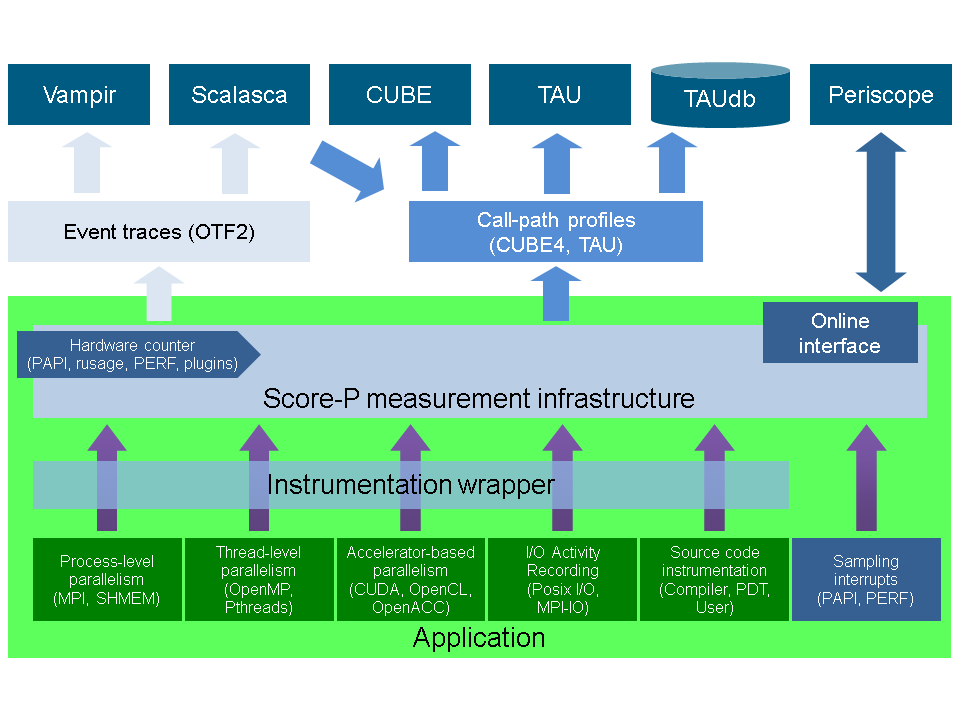
\includegraphics[scale=0.5]{Images-Rapport/score-p-overview.png}
\caption{Schéma de représentation de l'infrastructure Score-P et de ses interactions avec d'autres outils de profiling et de tracing d'applications HPC. \cite{score-p-doc}}
\label{schéma_scorep}
\end{center}
\end{figure}

Dans les grandes lignes, Scalasca suit le parcours suivant :
\begin{itemize}
\item le code est instrumenté (automatiquement ou manuellement) à l'étape de compilation en ajoutant simplement une commande wrapper de Score-P avant le compilateur. Par exemple \textit{mpicxx myapp.cpp -o myapp.exe} devient simplement \textit{scorep mpicxx myapp.cpp -o myapp.exe},
\item le code est mesuré et analysée avec \textit{scalasca -analyse mpiexec ...} au moment de l'exécution du code,
\item cette mesure est étudiée grâce à \textit{scalasca -examine <dossier\_experience>}, et l'interface graphique de Cube prend le relais pour un affichage et une étude simplifiés. Des optimisations (comme des filtres sur les fonctions mesurées) peuvent être ajoutés, tout comme la possibilité d'enregistrer la trace de l'application. Le schéma \ref{schéma_scorep_opti} présente ce cycle.
\end{itemize}

\begin{figure}
\begin{center}
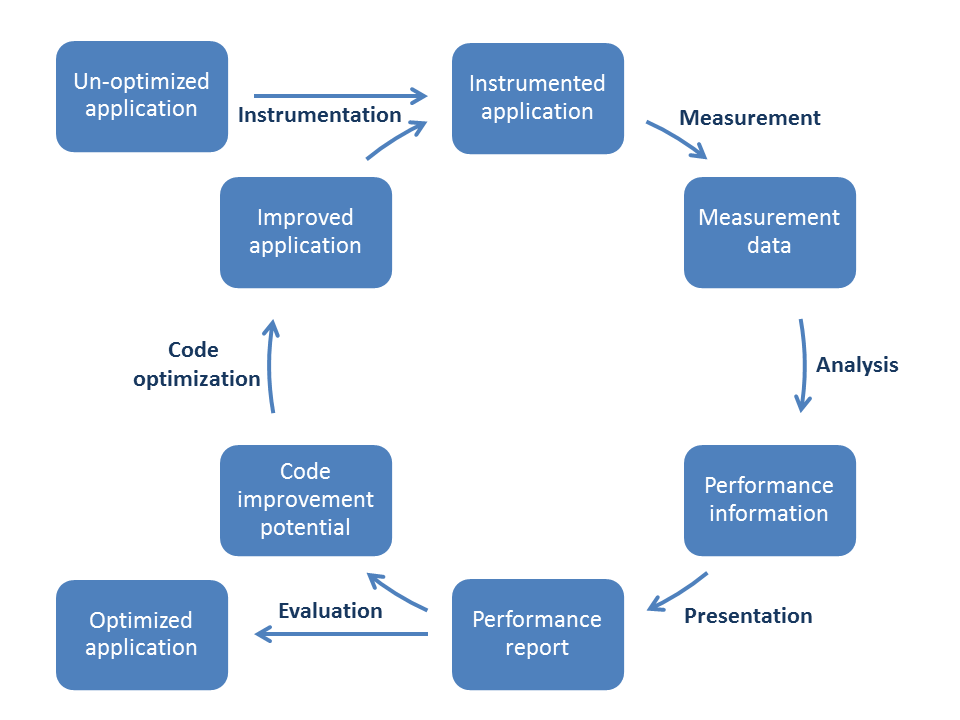
\includegraphics[scale=0.4]{Images-Rapport/perf-opt-cycle.png}
\caption{Cycle d'optimisation d'une application par mesures successives avec un outil comme Score-P. \cite{score-p-doc}}
\label{schéma_scorep_opti}
\end{center}
\end{figure}


\section{\'Etude de l'efficacité de l'optimisation avec Scalasca}

La mesure de miniXyce qui a été faite prend en paramètre le circuit cirRLC10 (10 échelons) car elle présente des résultats qui ne descendent pas en dessous de $10^{-11}$ comme cela a pu être constaté avec cirRLC100 par exemple. L'instrumentation automatique ne s'étant pas activée comme voulu, j'ai ajouté des mesures sur les trois fonctions de la zone critique MPI (à savoir \textit{gmres}, \textit{norm} et \textit{sparse\_matrix\_vector\_product}). L'overhead causé par l'appel à Scalasca augmente significativement le temps d'exécution, mais il permet tout de même d'avoir un aperçu des points chauds du code.\bigskip

\begin{figure}
\begin{center}
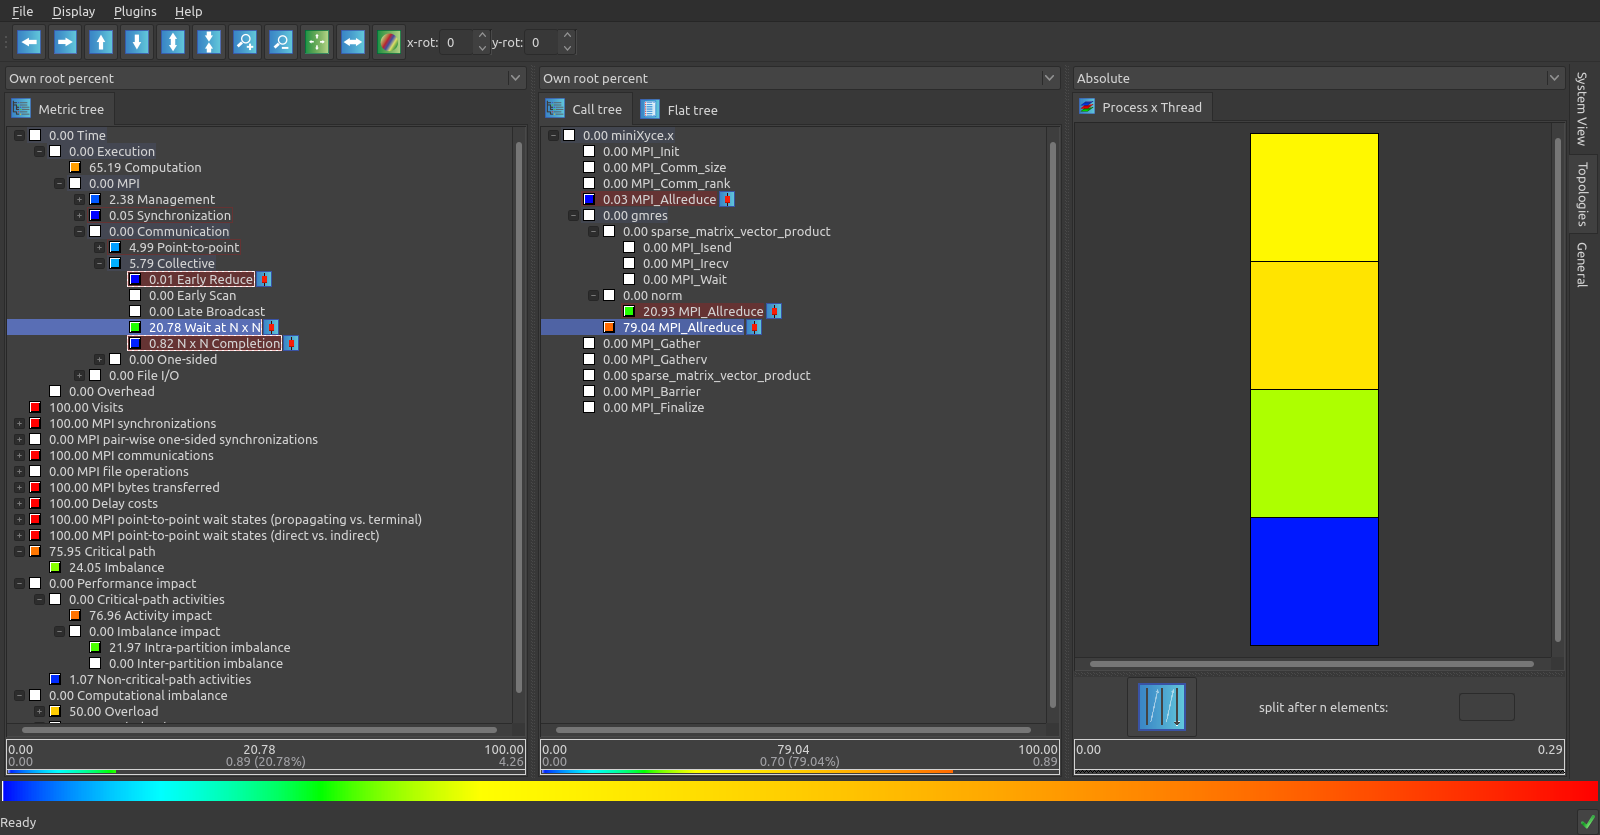
\includegraphics[scale=0.3]{Images-Rapport/cubeGUI.png}
\caption{Affichage du profil et de la trace de miniXyce avec 4 processus sur le circuit cirRLC10, grâce à l'interface graphique de CubeGUI.}
\label{cubeGUI}
\end{center}
\end{figure}

Sur la figure \ref{cubeGUI}, nous pouvons avoir un aperçu de l'analyse proposée par Scalasca. CubeGUI étant dynamique dans son utilisation, une seule image ne suffit pas à résumer toutes les informations que l'on peut tirer : sur le panneau de gauche, les principales mesures sont présentées avec un pourcentage du temps sur la branche considérée ainsi qu'une couleur (pour faciliter la lecture et avoir un ordre d'idée de l'importance de la donnée dans la branche). Ces couleurs se retrouvent sur le panneau de droite, qui distingue la métrique suivant chacun des processus en jeu (sur la figure \ref{cubeGUI}, il y en a 4, et les processus 0 et 1 sont bien plus concernés par la métrique sélectionnée que le processus 3). Enfin, le panneau central fait aussi la distinction suivant les fonctions dans lesquelles le problème est le plus rencontré. Par exemple sur notre capture, nous étudions spécifiquement les appels à MPI\_Allreduce issus de la fonction \textit{gmres}.

Voici les conclusions que nous pouvons tirer de cette étude :
\begin{itemize}
\item en termes de communications MPI (qui représentent 34.81\% du temps d'exécution), MPI\_ Allreduce est très présent, autant en occurrences ($127.000$ dans \textit{gmres} mais en dehors de \textit{norm}) qu'en temps (27.40\% du temps total de la simulation). Par ailleurs, Scalasca ne présente pas les MPI\_Wait comme vraiment problématiques, bien qu'il relève un désordre dans les envois et réceptions qui ralentit tout de même un peu.
\item l'attente au niveau des Allreduce est en réalité en majorité causé par P3 : il semblerait qu'il soit le dernier à rejoindre les autres processus sur ces communications collectives. Cette observation est cruciale puisqu'elle soulève un second problème analysé par Scalasca : le déséquilibre des charges de calcul entre processus.

En effet, il a toujours été supposé que chacun des processus avait un nombre quasi-équivalent de multiplications à effectuer. Mais dans le cas cirRLC10 par exemple, la matrice $A$ comporte une partie relativement tri-diagonale, puis deux autres "diagonales inclinées" qui se rejoignent vers le coin inférieur droit de la matrice sans pour autant s'atteindre. Ainsi, P3 a beaucoup plus de valeurs à recevoir et à envoyer, mais très peu de valeurs sur son blocs diagonal (moitié moins que P0 et P1). Il est donc normal qu'il soit le dernier à terminer son produit matrice-vecteur et à être attendu par les autres processus, ce qui rompt totalement la possibilité de rendre le code scalable.
\end{itemize}


\section{Comment rendre miniXyce scalable ?}

Ce qu'une lecture du code de \textit{gmres} nous indique, c'est que les parties de synchronisations sont très présentes et régulières : les processus n'ont pas réellement le temps de profiter de leur marge de liberté par rapport aux autres, et le déséquilibre des charges relevé n'y aide pas. Alors, que faire ?\bigskip

Il serait envisageable de repenser le code, même avec des envois bloquants, de façon profonde. Jocelyne Erhel \cite{erhel95} propose ainsi un découpage de la matrice dans la lignée de ce que nous avons proposé mais utilise des communications bloquantes. Ses résultats montrent une bonne scalabilité forte jusqu'à un certain seuil. Nous pourrions ainsi retravailler le code dans cette idée.\medskip

Nous pourrions aussi nous restreindre à la matrice considérée et chercher un découpage optimal des lignes entre les processus, de sorte à minimiser les appels à MPI et maximiser les calculs diagonaux. Cette approche est néanmoins trop spécifique à un problème donnée et ne s'inscrit pas dans la logique des miniapps de proposer une optimisation globale à une application préexistante.\medskip

Enfin, un changement de paradigme de programmation serait envisageable. \'Etant donné le nombre important d'échanges entre processus sur des valeurs, nous pourrions imaginer qu'ils partagent ces données et ne se synchronisent que lors de calculs sur une donnée globale, comme lors du calcul de la norme d'un vecteur. Le partage de travail équitable pourrait se faire plus facilement en partant du principe qu'un worker ayant terminé une ligne pourrait s'occuper d'une autre (et potentiellement travailler sur plus de lignes qu'un autre worker) tout en réduisant le temps global de calcul. Le stockage mémoire reste le même et devrait même être réduit du fait que les \textit{send\_instructions} et \textit{recv\_instructions} ne sont plus nécessaire (bien que des implémentations de sections critiques nécessitent des objets d'exclusion mutuelle).

L'approche proposée est celle de la \textbf{programmation sur machine à mémoire partagée}, en exploitant les API \textbf{OpenMP} ou \textbf{Pthreads}. Un scheduling dynamique du partage des lignes est donc tout à fait approprié. L'inconvénient majeur d'une implémentation OpenMP que je relève à ce stade serait la restriction vis-à-vis de la machine cible : si plusieurs nœuds SMP ou NUMA sont disponibles sur un calculateur, nous devrons nous contenter d'un seul d'entre eux, du fait que les threads ne se partageront pas les données de façon distante. Un hybride MPI+OpenMP serait alors nécessaire, avec la faible performance que nous lui connaissons pour l'instant. Il faut raison garder : miniXyce ou Xyce peuvent se trouver en majorité exécutés sur de petits calculateurs, ou même des ordinateurs personnels (laptop/desktop) qui ne peuvent apporter qu'un nombre limité de threads mais en mémoire totalement partagée.






\chapter{Refactoring OpenMP}

Suite au travail précédent, je me suis engagé dans un travail de fond afin d'améliorer significativement les performances du code : réécrire la partie solveur du code en OpenMP.

Lors d'une première tentative, j'ai entrepris de modifier à la volée les parties du code nécessitant des transformations. Mais devant l'instabilité du code créé (variables partagées devant être "remontées" hors de leur fonction, push\_back des vecteurs non adaptés à la mémoire partagée, ...), une compréhension plus profonde du fonctionnement de la méthode GMRES ainsi que de son implémentation dans miniXyce était primordiale.

Dans ce chapitre, nous présenterons ainsi dans un premier temps les fondements mathématiques de la méthode GMRES avec redémarrage sans pré-conditionnement, en s'appuyant sur l'implémentation de miniXyce. Nous détaillerons ensuite la méthode qui a été menée pour obtenir un code OpenMP modulaire obtenant des résultats valides, au travers d'un développement guidé par les tests. Enfin, nous présenterons les mesures de temps effectuées (scalabilité et profil de comparaison avec la version séquentielle d'origine), le gain obtenu ainsi que les améliorations encore possibles (scheduling et barrières).


\section{La méthode GMRES avec redémarrage}

\subsection{Notations}

Posons les bases du problèmes. Considérons un système linéaire de taille $N \in \N^*$ de la forme :
\[
A\vec{x} = \vec{b}
\]
avec $A \in \mathcal{M}_{N \times N}(\R)$ une matrice carrée creuse inversible, et $\vec{b} \in \R^N$ un vecteur. Le système possède une unique solution.\medskip

Soit $\vec{x_0} \in \R^N$ un vecteur quelconque, nommé "vecteur initial". En pratique, il est courant de prendre $\vec{x_0} = \vec{0}$. Le résidu initial $\vec{r_0} := \vec{b} - A \cdot \vec{x_0}$ et sa norme $\lVert \vec{r_0} \rVert$ donnent une première idée de l'erreur commise en choisissant $\vec{x_0}$.

$\vec{x_0}$ sert de point de départ à la méthode GMRES, vue comme une méthode itérative. En réalité, cette méthode converge vers une solution exacte du problème en au plus $N$ étapes, mais ce qui fait sa force est le fait qu'en pratique, seul un nombre d'étapes assez petit devant $N$ est nécessaire pour atteindre une convergence "convenable".\medskip

Pour quantifier ce "convenable", nous définissons ainsi $\epsilon$ comme étant la tolérance : une solution approchée $\vec{x}$ telle que le résidu $ \vec{r}_{\vec{x}} := \lVert \vec{b} - A \cdot \vec{x} \rVert \leq \epsilon$ sera considérée comme suffisamment proche de la solution exacte.\medskip

D'autre part, considérons le k-ième espace de Krylov engendré par $A$ et $\vec{r_0}$ :
\[
\mathcal{K}_k (A,\vec{r_0}) := \text{vec}\left\{ \vec{r_0}, A\vec{r_0}, A^2 \vec{r_0}, ..., A^k \vec{r_0} \right\} \quad\text{, avec } k \in \N
\]

\subsection{Procédé d'orthonormalisation d'Arnoldi}

En pratique, les vecteurs de la base de Krylov ont tendance à être proches de la dépendance linéaire, c'est pourquoi on applique un procédé d'orthonormalisation afin d'améliorer la stabilité numérique en obtenant une base orthonormée. La méthode d'Arnoldi s'appuie sur la méthode de Gram-Schmidt pour nous fournir une telle base $\vec{v_0}, \vec{v_1}, ..., \vec{v_i}, i \in \N^*$ (avec $i \leq k$ en général, car rien ne nous assure que la dimension du k-ième espace de Krylov soit égale à $k+1$).\medskip

\underline{\textbf{Remarque :}} Il existe plusieurs façons de concevoir GMRES, notamment pour trouver une base orthonormée de l'espace de Krylov, mais nous nous contenterons de notre approche.\bigskip

\underline{\textbf{Algorithme :}}
Une itération $i$ d'Arnoldi se déroule de la manière suivante :
\begin{itemize}
\item Pour $i=0$,
\[
\vec{v_0} := \frac{\vec{r_0}}{\lVert \vec{r_0} \rVert}
\]
\item Pour $i \neq 0$, calculer les produits scalaires :
\[
\begin{array}{l}
h_0 := <\vec{v_0},A\vec{v_{i-1}}>, \\
h_1 := <\vec{v_1},A\vec{v_{i-1}} - h_0\vec{v_0}>, \\
\vdots \\
h_{i-1} := <\vec{v_{i-1}},A\vec{v_{i-1}} - h_0\vec{v_0} - h_1 \vec{v_1} - ... - h_{i-2} \vec{v_{i-2}}> \\
\end{array}
\]
\item Calculer la norme :
\[
\begin{array}{l}
h_i := \lVert A\vec{v_{i-1}} - h_0 \vec{v_0} - ... - h_{i-2} \vec{v_{i-2}} \rVert
\end{array}
\]
\item Le nouveau vecteur $\vec{v_i}$ de la base est :
\[
\begin{array}{l}
\vec{v_i} := \frac{A\vec{v_{i-1}} - h_0 \vec{v_0} - ... - h_{i-2} \vec{v_{i-2}}}{h_i}
\end{array}
\]
\end{itemize}

Ainsi, à chaque étape d'Arnoldi, nous agrandissons la nouvelle base orthonormée en prenant en compte un vecteur de la base d'origine supplémentaire. Dans le contexte d'une méthode itérative (donc pour laquelle on ne sait pas à l'avance le nombre d'itérations que l'on va réaliser) cette méthode est adaptée, mais comme le précise Erhel \cite{erhel95}, il y a une forte dépendance entre une étape et la suivante. 

Précisons par ailleurs que la mise à jour avec les soustractions peut théoriquement se faire après le calcul de tous les $h_i$ par bilinéarité du produit scalaire et orthogonalité des $\vec{v_i}$ (les produits scalaires deviennent $h_0 = <\vec{v_0}, A \vec{v_{i-1}}>$, etc.).\medskip

D'autre part, en stockant à chaque étape les coefficients $h_i$ dans une colonne (et en remplissant les lignes éventuellement manquantes par des zéros), nous pouvons former une matrice qui est, par construction, une matrice de Hessenberg supérieure non-carrée ($i+1$ lignes et $i$ colonnes) :
\[
H_i := \left(
\begin{matrix}
h_0^1  & h_0^2  & ... & h_0^i \\
h_1^1  & h_1^2  & ... & h_1^i \\
0      & h_2^2  & ... & h_2^i \\
0      & 0      & ... & h_3^i \\
\vdots & \vdots & ... & \vdots \\
0      & 0      & ... & h_i^i \\
\end{matrix}
\right)
\]
où l'exposant représente l'étape $i$ d'Arnoldi à laquelle le produit scalaire a été calculé.

\begin{theorem}\label{theoreme_arnoldi}
\[
\forall i \in \N^*, A V_i = V_{i+1} H_i \text{\quad, avec } V_i = \left( \begin{matrix}
\vec{v_0} | \vec{v_1} | ... | \vec{v_i}
\end{matrix} \right)
\]
\end{theorem}
La démonstration se fait par récurrence sur $i$.\medskip

\underline{\textbf{Remarque :}} Si, à une étape $i$ donnée, le nombre de vecteurs dépasse la dimension maximale de l'espace de Krylov, alors $h_i$ sera nul. Dans ce cas, il faudra ajouter une vérification dans notre implémentation afin de ne pas créer le vecteur $\vec{v_i}$ (qui est simplement le vecteur nul). Aucune autre sécurité n'est à mettre en place puisque, comme nous allons le voir dans la section suivante, le sinus de la rotation de Givens associée sera aussi égal à $0$, ce qui garantit que nous avons atteint la solution exacte (et que GMRES est terminé). 

\subsection{Factorisation QR, rotations de Givens et minimisation des résidus}

Pour la suite, nous allons avoir besoin de connaître la factorisation QR de $H_i$ car des résolutions de systèmes impliquant $H_i$ vont avoir lieu, et l'apparition d'une matrice triangulaire supérieure $R$ sera alors bénéfique.

Nous obtenons ainsi le théorème suivant (reformulé à partir de \cite{gmres_wikipedia}) :

\begin{theorem}
~\\
$\forall i \in \N^*, H_i = Q_i R_i$
est la décomposition QR de $H_i$, avec $Q_i \in \mathcal{M}_{(i+1)\times(i+1)}$ orthogonale et $R_i \in \mathcal{M}_{(i+1)\times i}$ triangulaire supérieure (avec des coefficients positifs sur la diagonale), telles que :
\[
Q_i = (G_i \cdot G_{i-1} ... G_2 \cdot G_1)^T, \text{ avec $G_j$ une matrice de rotation de Givens associée aux lignes $j$ et $j+1$}
\]
et
\[
R_i = \left( \begin{matrix}
R_{i-1} & \vec{\eta}_i \\
0 ... 0 & 0 \\
\end{matrix} \right), \text{ avec } \vec{\eta}_i = G_i \cdot G_{i-1} ... G_2 \cdot G_1 \cdot \left( \begin{matrix}
h_0^i \\
\vdots \\
h_i^i
\end{matrix} \right) \text{ et $R_0$ la matrice vide}
\]

De plus,
\[
G_j = \left( \begin{matrix}
1 \\
 & \ddots \\
 &       & c_j    & s_j \\
 &       & -s_j   & c_j \\
 &       &        &     & \ddots \\
 &       &        &     &       & 1 \\
\end{matrix} \right), \text{ où les $c_j$ sont sur les $j$-ième et $(j+1)$-ième lignes}
\]

avec $c_i = \frac{\rho_i}{\sqrt{\rho_i^2 + \sigma_i^2}}$ est le cosinus de la matrice et $s_i = \frac{\sigma_i}{\sqrt{\rho_i^2 + \sigma_i^2}}$ est le sinus, en posant $\rho_i$ et $\sigma_i$ l'avant-dernière et la dernière composante de $G_{i-1} ... G_2 \cdot G_1 \cdot \left( \begin{matrix}
h_0^i \\
\vdots \\
h_i^i
\end{matrix} \right)$
\end{theorem}
\noindent La démonstration se fait aussi par récurrence (cf \cite{gmres_wikipedia}).\medskip

Les dimensions des matrices de Givens ne sont pas explicitement données dans le théorème car elles sont amenées à changer au fur et à mesure des itérations, en ajoutant simplement une ligne de matrice identité. Elles conservent ainsi leur sens "physique" en tant que rotations, mais dans un sous-espace vectoriel plus grand. Les valeurs $\rho_i$ et $\sigma_i$ restent les avant-dernière et dernière valeurs dans la version restreinte du sous-espace (i.e. à l'itération $i$).

\`A noter aussi que les nouveaux cosinus et sinus pour une itération $i$ ne peuvent être calculés qu'en ayant connaissance de la dernière et de l'avant-dernière composante du vecteur $G_{i-1} ... G_2 \cdot G_1 \cdot \left( \begin{matrix}
h_0^i \\
\vdots \\
h_i^i
\end{matrix} \right)$ : en effet, ils sont "choisis" de sorte à éliminer la dernière composante de ce vecteur.

Par ailleurs, le théorème montre aussi que la matrice $R_i$ s'obtient à faible coût à partir de la matrice $R_{i-1}$ de l'étape précédente en accolant un nouveau vecteur, obtenu grâce à la dernière colonne de $H_i$ : nous voyons ainsi l'efficacité en termes de calculs que nous apporte cette décomposition.\bigskip

\underline{\textbf{Principe de GMRES :}}
Le principe de GMRES consiste à chercher la solution du système $A\vec{x} = \vec{b}$ en prenant comme solution approchée $\vec{x_i} := \vec{x_0} + V_i \vec{y_i}$, avec $V_i$ la matrice définie dans le théorème \ref{theoreme_arnoldi} et $\vec{y_i} \in \R^i$, de sorte à minimiser la norme du résidu : $\lVert \vec{r_i} \rVert := \lVert b - A \cdot \vec{x_i} \rVert$. Cette minimisation est un problème des moindres carrés pour lequel le théorème suivant fournit une méthode de résolution :

\begin{theorem}
\[
\forall i \in \N^*, \lVert \vec{r_i} \rVert = \lVert H_i \vec{y_i} - \lVert \vec{r_0} \rVert e_1^i \rVert = \lVert R_i \vec{y_i} - \vec{g_i} \rVert
\]

avec : $e_1^i = \left( \begin{matrix}
1\\
0\\
\vdots\\
0
\end{matrix} \right) \in \R^{i+1}$ et $\vec{g_i} := \lVert \vec{r_0} \rVert Q_i^T e_1^i \in \R^{i+1}$

De plus, la dernière composante de $\vec{g_i}$ est égale à $\underset{\vec{r_i} \in \R^N}{\min} \lVert \vec{r_i} \rVert$.
\end{theorem}

Ainsi, résoudre le problème de minimisation revient à trouver la solution $\vec{y_i}$ du système triangulaire supérieur $\R_i \vec{y_i} = \vec{g_i}$ \underline{\textbf{en supprimant la dernière ligne du système}} (i.e. les zéros de $R_i$ et la dernière composante, censée être proche de 0, de $\vec{g_i}$).

Il est important de noter que, même s'il change de taille, le vecteur $\vec{g_i}$ est facilement mis à jour à partir du vecteur précédent et des rotations de Givens : il suffit en effet d'ajouter une nouvelle composante en "clonant" la dernière et en la multipliant par $-s_i$. Il faut aussi multiplier l'ancienne dernière composante (qui est maintenant l'avant-dernière !) par $c_i$.\medskip

Enfin, la dernière composante de $\vec{g_i}$ nous donne la valeur de l'erreur commise sur la solution approchée sans avoir besoin de résoudre le système triangulaire $R_i y_i = g_i$ : c'est cette remarque qui va nous permettre d'itérer un certain nombre de fois jusqu'à obtenir une valeur inférieure à notre tolérance $\epsilon$, sans perdre de temps à résoudre un système intermédiaire.

\subsection{Redémarrage}

Comme nous l'avons dit, GMRES convergera vers la solution exacte du problème en au plus $N$ étapes, mais en pratique, il est attendu qu'elle converge vers une valeur très proche en un nombre d'étapes petit par rapport à $N$.

Cependant, il existe des situations pour lesquelles la convergence est très lente (i.e. que les résidus diminuent très peu au fil des itérations, voire ne diminuent pas) jusqu'à la dernière itération où la convergence se fait en une seule itération.

Pour éviter ce genre de problèmes où les calculs successifs sur chaque étape ne nous apportent aucun gain sur les résidus, une politique de redémarrage peut être prise : elle consiste à fixer en avance une dimension maximale $k \in \N^*$ de l'espace de Krylov et à considérer que l'erreur doit devenir plus petite que la tolérance en moins de $k$ itérations.

Si ce n'est pas le cas, alors on estime que le point de départ $\vec{x_0}$ était mauvais. Ainsi, on abandonne la base $\vec{v_0}, \vec{v_1}, ...$ construite et on recommence la construction avec un nouveau vecteur initial. Le choix de ce vecteur initial peut être fait à partir de $\vec{x_k}$ (l'approximation de $\vec{x}$ qui aurait été prise si le résidu était assez petit).\bigskip

Choisir une valeur de $k$, assez grande pour ne pas redémarrer la méthode alors qu'une bonne solution était en vue, mais aussi assez petite pour éviter les calculs inutiles dans les situations mal engagées, nécessite une connaissance a priori de la matrice $A$ ou s'inscrit dans un choix arbitraire. Nous ne détaillerons pas davantage les méthodes de choix de ce paramètre et ferons simplement des essais lors des expérimentations. Gardons seulement en mémoire que $k$ est sensé être petit (voire très petit) devant $N$.


\subsection{Algorithme GMRES}

Maintenant que les concepts ont été formalisés mathématiquement, développons l'aspect algorithmique de la méthode GMRES. Je l'ai partagée en 5 étapes pour une meilleure compréhension :

\begin{itemize}
\item \underline{\textbf{\'Etape 1 :}} Initialisation

Calcul de l'erreur initiale : $err \leftarrow \lVert \vec{r_0} \rVert$

Mise à jour de la solution : $\vec{x} \leftarrow \vec{x_0}$\medskip

Si $err \leq tolerance$ : fin de l'algorithme.

Sinon, passer à l'étape 2.\medskip

\item \underline{\textbf{\'Etape 2 :}} Début du restart

Création de $\vec{v_0} \leftarrow \frac{\vec{b} - A\cdot \vec{x}}{\lVert \vec{b} - A\cdot \vec{x} \rVert}$, première colonne de la matrice $V$

La première composante de $\vec{g}$ devient $\lVert \vec{r_0} \rVert$.\medskip

\item \underline{\textbf{\'Etape 3 :}} Itération $i$ d'Arnoldi

Calcul des composantes $h_0, h_1, ..., h_i$ de la nouvelle colonne de la matrice $H$

Création du nouveau vecteur $v_i$, la nouvelle colonne de la matrice $V$\medskip

\item \underline{\textbf{\'Etape 4 :}} Rotations de Givens à l'itération $i$

Appliquer les rotations de Givens $G_1, G_2, ..., G_{i-1}$ (dans cet ordre) à la nouvelle colonne de $H$

Calculer le cosinus et le sinus de la nouvelle rotation, puis l'appliquer à la colonne de $H$

Mettre à jour $\vec{g}$ en lui appliquant la nouvelle rotation de Givens

Mettre à jour $err \leftarrow | \text{dernière composante de } \vec{g} |$\medskip

Si $err \leq tolerance$ ou $i > k$, passer à l'étape 5.

Sinon, revenir à l'étape 3 avec $i \leftarrow i+1$.\medskip

\item \underline{\textbf{\'Etape 5 :}} Mise à jour de $\vec{x}$

Résoudre le système triangulaire $R \vec{y} = \vec{g}$ (sans la dernière ligne)

Mise à jour de la solution : $\vec{x} \leftarrow \vec{x} + V \cdot \vec{y}$ (sans la dernière colonne de $V$)\medskip

Si $err \leq tolerance$ : fin de l'algorithme

Sinon, revenir à l'étape 2.
\end{itemize}\bigskip

Les matrices $H$ et $R$ sont confondues dans l'algorithme étant donné que $R$ est le résultat de l'application de rotation de Givens sur $H$ : en mémoire de l'ordinateur, elle ne seront pas stockées de façon disjointes mais $R$ "écrasera" $H$ (étant donné que seul $R$ nous intéresse).



\section{Implémentation de GMRES en OpenMP}

\subsection{Méthode de conception adoptée}

Même si l'implémentation MPI proposait globalement la même structure que celle présentée, elle présentait le désavantage d'être difficile à lire et non adaptée à une réécriture en OpenMP. Plusieurs modifications significatives ont été apportées :

\begin{itemize}
\item La première d'entre elles a été de concevoir des fonctions très simples mais souvent utilisées : le produit scalaire, le GAXPY et le SAXPY. La norme étant une racine carrée d'un produit scalaire, il n'était pas nécessaire d'en faire une fonction à part. Le GAXPY est sous la forme classique proposée par la bibliothèque BLAS, à ceci près qu'il a besoin d'un réceptacle supplémentaire et ne réécrit pas sur les variables d'entrées (sauf le réceptacle prévu spécifiquement pour le résultat). Il en est de même pour le SAXPY. Par ailleurs, le GAXPY est adapté à la structure de matrice creuse présente dans le code.

Ces trois fonctions sont censées être appelées dans une région parallèle par tous les threads : le partage de travail sur les réductions et les instructions For permet un gain de temps.

\item 4 autres fonctions correspondant aux étapes 3, 4 et 5 sont ajoutées pour accentuer davantage la modularité du code : une itération d'Arnoldi, les applications des rotations de Givens et la mise à jour de $\vec{g}$ et de l'erreur, la résolution d'un système triangulaire, et enfin la mise à jour du vecteur $\vec{x}$.

L'intérêt de ces fonctions, en plus d'une lisibilité et d'une maintenabilité augmentée du code, réside dans le fait qu'elles encapsulent les caractéristiques des paramètres. En effet, les matrices et vecteurs ont une taille déjà fixée à l'avance (cf point suivant) ce qui nécessite une manipulation attentive, dépendante de l'itération à laquelle on se trouve : par exemple, un vecteur prévu à une taille de 4 peut, dans le cas d'un système simple à résoudre, n'être exploité que jusqu'à sa 3 coordonnée. Si une boucle venait à parcourir l'ensemble du vecteur, des valeurs non-initialisées viendraient perturber le déroulement de l'algorithme (et fournir des résultats erronés).

\item En complément de la conception de toutes ces fonctions, des tests unitaires ont été développés de sorte à se détacher du problème initial et s'assurer que sous les conditions seules de tailles de matrices/vecteurs, la fonction faisait ce que l'on attendait d'elle.

Cette conception orientée par les tests a permis de débusquer de nombreux bugs, en complément d'outils comme GDB (GNU Debugger), et de tester le comportement sur des valeurs autres que celles fournies par les circuits de miniXyce.

En complément, de très nombreux commentaires parsèment le code pour simplifier sa compréhension, et l'utilisation d'asserts (fournis par la libC) accentue la robustesse du code. Ces asserts, gourmands en temps d'exécution, peuvent être désactivés à la compilation (-DNDEBUG en flag de compilation) lorsque la validité du code est assurée.

\item Afin d'éviter de travailler sur de petites régions parallèles fréquentes, l'implémentation que nous proposons est à gros grains ("coarse grain") : au niveau de la partie transitoire, une unique région parallèle est créée, et les fonctions étant appelées en séquentiel le sont à l'intérieur d'un \textit{pragma omp single}.

Une écrasante majorité des variables est partagée, dont une structure \textbf{Storage\_GMRES} contenant 6 variables :
\begin{itemize}
\item 2 vecteurs contenant les cosinus et sinus successifs des rotations de Givens,
\item un vecteur $\vec{g}$
\item un vecteur $\vec{y}$
\item et deux vecteurs de vecteurs (i.e. des matrices) $R$ et $V$
\end{itemize}

Cette structure possède deux intérêts : réunir en une seule structure des variables partagées entre les threads et ayant un statut de variable de travail, mais aussi encapsuler leur utilisation et leur initialisation (notamment leurs tailles). Ce second point est réalisé par le constructeur de la classe, qui offre l'élégance de son utilisation et la robustesse (les vecteurs ne sont pas amenés à changer de taille en cours d'exécution).

Le choix de leur taille est fixé selon la variable $k$ correspondant à la dimension maximale de l'espace de Krylov : $k$ étant très supposé très petit devant $N$, même si une sur-évaluation de sa valeur a eu lieu (par exemple en prenant $k=10$ alors que la convergence s'effectue déjà à $k=3$), le gain en temps reste satisfaisant face à la perte en mémoire, qui reste très modérée.
\end{itemize}

Une remarque importante : a priori, au début de l'étape 2, nous sommes amenés à recalculer la norme du résidu au cas où nous soyons dans un redémarrage. En pratique, sur les circuits proposés, le redémarrage semblait peu présent, ce qui a motivé l'ajout d'une condition If. On vérifie si nous sommes au cœur d'un redémarrage et si ce n'est pas le cas (i.e. la première fois que l'on passe par cette étape), alors on évite ce calcul redondant en récupérant la norme au travers de $err$. En stockant $\vec{r_0}$ dans $V$ dans l'emplacement de $\vec{v_0}$ (temporairement), nous économisons tous les calculs de cette étape.


\subsection{Complexité spatiale et temporelle}

\underline{\textbf{Complexité mémoire :}}

En ne considérant que la structure \textit{Storage\_GMRES} (les autres variables prenant bien moins de place), nous observons que les vecteurs des sinus et cosinus prennent chacun $k$ flottants double précision, tout comme $\vec{y}$. $\vec{g}$ en prend quant à lui un de plus.

Pour les matrices, $V$ est pleine de $k+1$ vecteurs de taille $N$, alors que $R$ (qui stocke $H$ au début) est de Hessenberg rectangulaire, ce qui correspond à $1+2+ ... + k + k$ flottants double précision, soit $k \frac{k+3}{2}$ flottants.

\textbf{Total :} Le stockage prend $4k+1+k \frac{k+3}{2} + N(k+1)$ flottants double précision, ce qui correspond à $\underline{\mathcal{O}(k^2 + Nk)}$.\medskip

\underline{\textbf{Complexité en temps d'exécution :}}

\'Etudions la complexité du code en séquentiel. L'étape 1 nécessite le calcul d'une norme, ce qui correspond à une racine carrée et à un produit scalaire ($n$ multiplications et $n-1$ additions pour deux vecteurs de taille $n$). Il y a aussi une copie de vecteur ($\vec{x} \leftarrow \vec{x_0}$) et un GAXPY avec une matrice creuse ($\vec{b} - A \cdot \vec{x}$). Nous comptons $N$ opérations pour la copie et $2N$ pour la norme (en supposant que toutes ces opérations prennent autant de temps, ce qui n'est en pratique pas le cas notamment pour la racine carrée).

En notant $m$ le nombre moyen d'éléments non nuls par ligne de la matrice $A$, le GAXPY creux prend $mN$ multiplications, $(m-1)N$ additions et $N$ soustractions, soit un total de $2mN$ opérations.

\textbf{Total étape 1 :} $N(2m+3)$ opérations\medskip

L'étape 2 (lorsqu'elle est faite) recalcule $\vec{r_0}$ ($2mN$ opérations), sa norme ($2N$ opérations) et divise chaque composante par sa norme ($N$ opérations), ce qui équivaut à $(2m+3)N$ opérations.

L'étape 3 calcule un produit matrice vecteur ($(2m-1)N$ opérations), $i$ produits scalaires ($i(2N-1)$ opérations), une racine carrée ($1$ opération) et une division d'un vecteur par sa norme ($N$ opérations).

L'étape 4 calcule les nouveaux cosinus et sinus ($7$ opérations chacun), applique toutes les rotations ($6i-3$ opérations), met à jour $\vec{g}$ ($2$ opérations) et met à jour l'erreur ($1$ opération).

L'étape 5 résout un système triangulaire de taille au plus $k$ ($k^2$ opérations) et un GAXPY avec la matrice de taille au plus $N$ par $k$ ($2kN$ opérations).\bigskip

\textbf{Total opérations :} En comptant au maximum $k$ itérations, aucun redémarrage et $m$ éléments non nuls en moyenne par ligne de $A$, nous obtenons $\underline{\mathcal{O}(mkN+k^2 N)}$. Si $k$ est constant quel que soit la taille de $N$, GMRES est de complexité linéaire, mais il semble plus probable de considérer qu'en pratique, $k$ sera dépendant de $N$.




\section{Résultats de performances}

% profil simple comparatif entre version séquentielle et version séquentielle OpenMP (amélioration rien qu'avec le if(restarts == 0)
% courbe de scalabilité forte et faible en OpenMP + courbe de l'accélération (speedup)

% peut etre nouvelle section : refaire une analyse avec MAQAO/Scalasca pour voir ce qui bloque une meilleure scalabilité + dire u'il faut supprimer des barrières implicites / rendre l'implémentation de GMRES moins séquentielle (en s'appuyant sur les travaux de Erhel) + changer le scheduling (dynamic ? static plus grand ? guided ?)






























\begin{vplace}[0.5]

\chapter*{Conclusion}
\addcontentsline{toc}{chapter}{Conclusion}



\end{vplace}







\begin{vplace}
\chapter*{Annexe}
\addcontentsline{toc}{chapter}{Annexe}

% texte à écrire ici

\end{vplace}




\nocite{*}
\bibliographystyle{plain}
\bibliography{Biblio_Stage_Robin_CAZALBOU}

\end{document}
